\chapter{Spectral Energy Distribution Analysis}\label{sed}

\section{SED Fitting Method}

In order to determine a dust mass, we use the IDL package MPFIT \citep{markwardt2009} to fit equation 

\begin{equation}\label{eq:mod_sed}
  S_\nu\left(T\right) = \frac{M\:\kappa_{\nu,0}}{D^2}\left(\frac{\nu}{\nu_0}\right)^{\beta+3} B_\nu\left(T\right)
\end{equation}

\noindent for the temperature, T, mass, M, and the emissivity index, $\beta$ while the opacity, $\kappa_{\nu, 0}$, distance, D, and reference wavelength, $\nu_0$ are held fixed.  The routine MPFIT utilizes the Levenberg-Marquardt algorithm.  This algorithm uses a combination of two minimization techniques (the steepest descent method and the Newton-Raphson Method) to determine the parameter combination that corresponds to a minimum in the $\chi^2$ space while maximizing the efficiency of the step sizes in each iteration \citep{burden2001}.  The algorithm begins by implementing the steepest descent method.  The way this technique works is it will follow the direction opposite to the largest gradient in order to traverse the $\chi^2$ space to locate a minimum.  As the set of solutions approaches a minimum, it will switch to the Newton-Raphson method to locate the best set of parameters by finding where the derivative at that point is closest to zero \citep{gavin2013}.  

In order for MPFIT to provide the most accurate fit, we establish a reasonable uncertainty for each of our data points, and determine a realistic set of starting points for the fitting.  The variance for our SCUBA-2 data is determined using

\begin{equation}\label{eq:sc2noi}
  \sigma^2 = \sigma_{obs}^2 + \sigma_{rms,sky}^2 + \sigma_{calib}^2
\end{equation}

\noindent such that $\sigma_{obs}$ is the noise determined by MAKEMAP, $\sigma_{rms,sky}$ is the RMS of the sky, and $\sigma_{calib}$ is the product of calibration uncertainty and observed flux for each observed wavelength.  The systemic calibration scaling factors are shown in Table \ref{tab:calib_fac}.

\begin{deluxetable}{cc}
%  \tabletypesize{\footnotesize}
  \tablecolumns{2}
  \tablewidth{0pt}
  \tablecaption{Systematic Calibration Uncertainties for SCUBA-2 and KINGFISH Observations\label{tab:calib_fac}}
  \tablehead{\colhead{Observation} & \colhead{Scaling Factor}}
    \startdata
      100$\mu$m & 3\% \\
      160$\mu$m & 5\% \\
      250$\mu$m & 7\% \\
      350$\mu$m & 7\% \\
      450$\mu$m & 12\% \\
      500$\mu$m & 7\% \\
      850$\mu$m & 8\% \\
    \enddata
\end{deluxetable} 

The variances for the KINGFISH data are determined in a similar fashion using 

\begin{equation}\label{eq:kinnoi}
  \sigma^2 = \sigma_{rms,sky}^2 + \sigma_{calib}^2.
\end{equation}

\noindent The observation error is excluded since the reported variance in the filtered images reflects the fake source image used and not the KINGFISH data set.

The nature of the Levinberg-Marquardt method leaves the solution vulnerable to converge at a local minimum rather than converging at the global minimum.  This is remedied by selecting reasonable initial conditions.  The initial conditions we used were  a modified blackbody with a temperature of 20 K, a dust emissivity index of 2, and a mass determined by 

\begin{equation}\label{eq:mass}
  \begin{split}
    M & = \frac{D^2 \: S_{250}}{\kappa_{\nu,0} \:  B_{250}\left(T\right)} \left(\frac{\nu}{\nu_0} \right)^{-\beta} \\
      & = 5.40 \times 10^5 \: S_{250} \; \left[M_\odot\right]
  \end{split}
\end{equation}

\noindent using the flux from the 250$\mu$m emission and our initial temperature and dust emissivity index values with a reference opacity of 0.2665 m$^2$ kg$^{-1}$ at 300$\mu$m.  When the best fit values have been calculated we use equation \ref{eq:mass} to determine the dust mass associated with the 250$\mu$m emission instead of using the fitted peak mass in order to increase the signal to noise of our data and avoid any temperature dependences associated with emission further from the Rayleigh-Jeans tail of the SED.  The error in the dust mass is then determined by taking the total derivative of the mass function with respect to each of the free variables.

\section{Fitting the Spectral Energy Distribution}

The fitting procedure was carried out in two different ways on a modified blackbody equation.  One of the two methods is fitting an SED to each individual pixel in order to generate a set of parameter maps.  The second method sums the flux of each of the selected regions shown in Figure \ref{fig:regions} to maximize the signal to noise ratio in order to generate a more precise set of parameters.  For both of the fitting methods the mass, $M$, and temperature, $T$, are set as free parameters, but the emissivity index, $\beta$, requires special treatment for each of the methods.  The distance, D, has been set to 9.4 Mpc \citep{walter2008}, and the reference opacity, $\kappa_{\nu,0}$, was tested using 0.2665 m$^2$ kg$^{-1}$ \citep{li2001} and 1.0 m$^2$ kg$^{-1}$ \citep{planckxxv2011}.

\begin{figure}
  \centering
  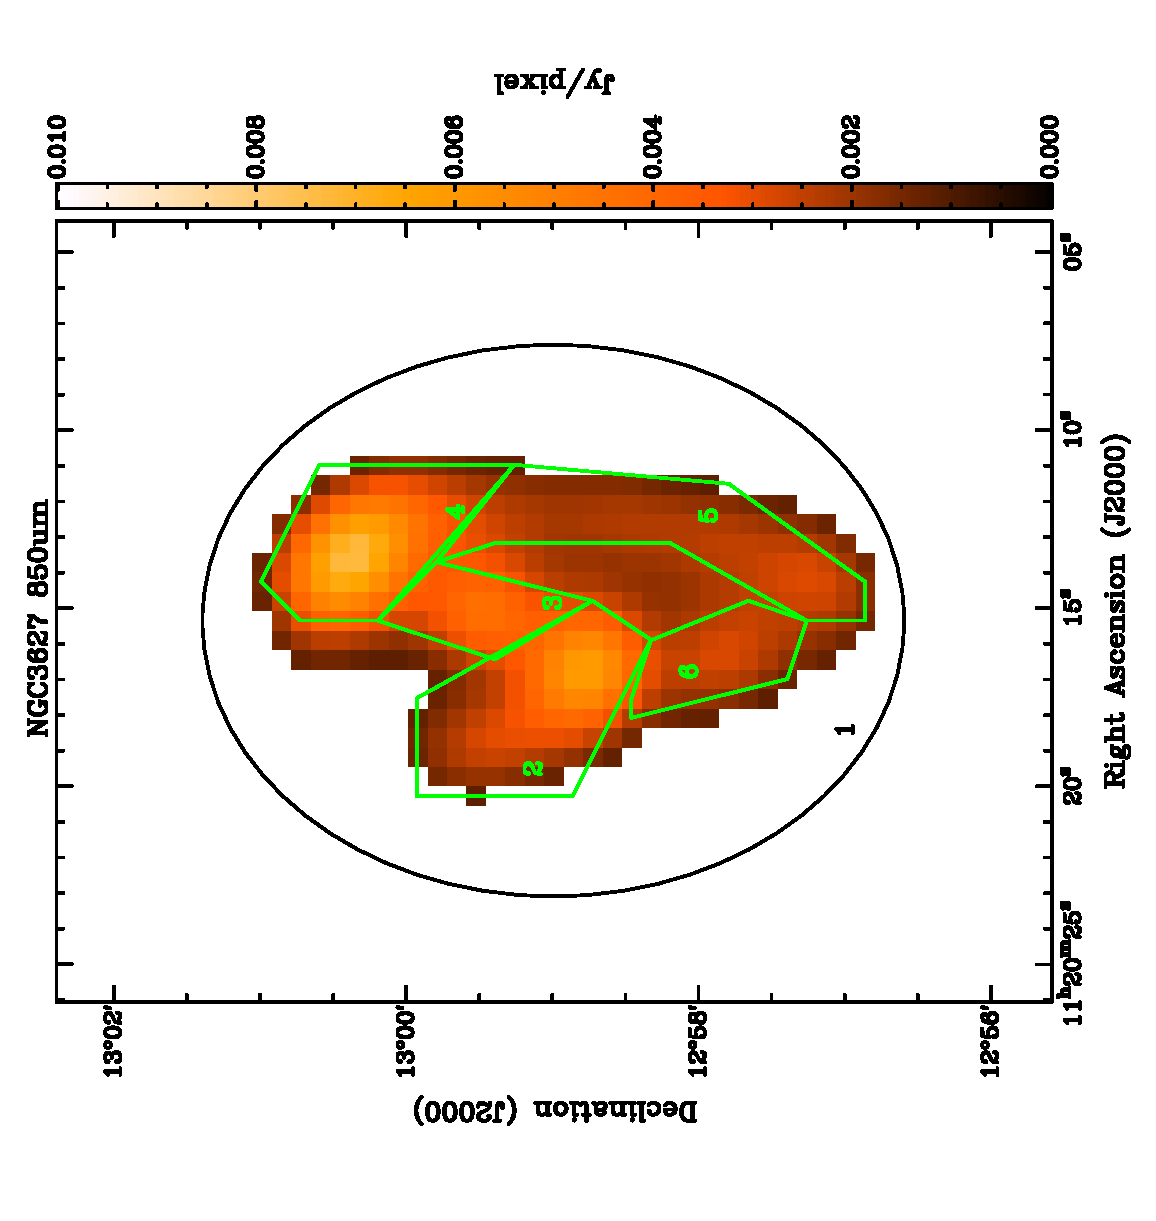
\includegraphics[width=1.\textwidth,angle=270]{sed_imgs/regions.eps}
  \caption[NGC3627 Regions]{850$\mu$m emission convolved to the 500$\mu$m beam size overlaid with the selected regions of NGC3627 labeled 1 through 6 such that region 1 includes the entire galaxy.}
  \label{fig:regions}
\end{figure}

\subsection{Pixel SED Fits}

In order to generate a parameter map of NGC3627, each individual pixel has its own SED determined from the available wavelengths described in the observations chapter.  The fits are performed over 100$\mu$m, 160$\mu$m, 250$\mu$m, 350$\mu$m, 450$\mu$m or 500$\mu$m, and 850$\mu$m observations.  Initially, we excluded the 500$\mu$m emission in order to increase the resolution of our final maps, but an over abundance of emission in the 450$\mu$m map provided unreliable results, so we exchanged the 450$\mu$m emission with 500$\mu$m emission.  The maps used in the SED fitting is shown in Figure \ref{fig:images} where each image has been convolved to the resolution of the 500$\mu$m observations and a 5$\sigma$ cut has been applied.  The treatment of the dust emissivity index is performed by fixing it at $\beta=1.8$ for the Planck opacity model where the opacity is $\kappa_{300\mu m,0}=1.0$ m$^2$ kg$^{-1}$ \citep{planckxxv2011} and $\beta=2.0$ for the Li and Draine opacity model where the opacity is $\kappa_{300\mu m,0}=0.2665$ m$^2$ kg$^{-1}$ \citep{li2001}.  A third fit is performed where the emissivity index is allowed to vary as a free parameter.  While the emissivity index is allowed to vary, the opacity being used is the Planck model.  Using either an opacity of 1.0 m$^2$ kg$^{-1}$ or 0.2665 m$^2$ kg$^{-1}$ will not affect the shape of the SED, only its normalization.  In the case of our fits, it is the mass that acts as the normalizing value, so increasing or decreasing the opacity will yield the opposite effect in the mass.  The inverse proportionality can be seen in equation \ref{eq:mass}.  

\begin{figure}
  \begin{subfigure}[t]{0.48\textwidth}
    \centering
    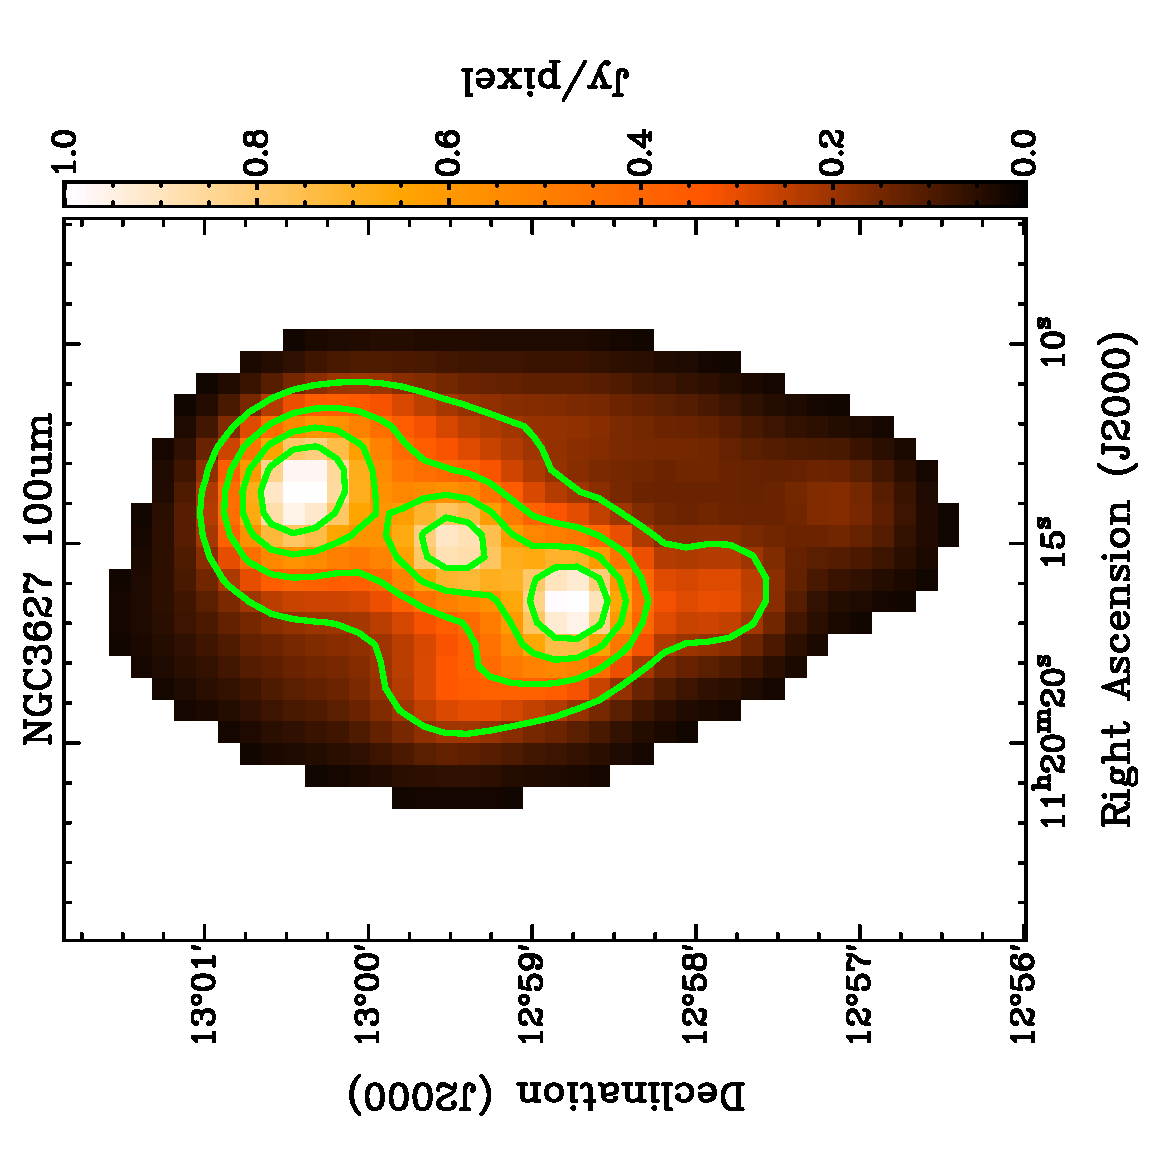
\includegraphics[width=1.\linewidth, angle=270]{sed_imgs/100_sed.eps}
%    \caption{100$\mu$m Observations}
  \end{subfigure}
  \quad
  \begin{subfigure}[t]{0.48\textwidth}
    \centering
    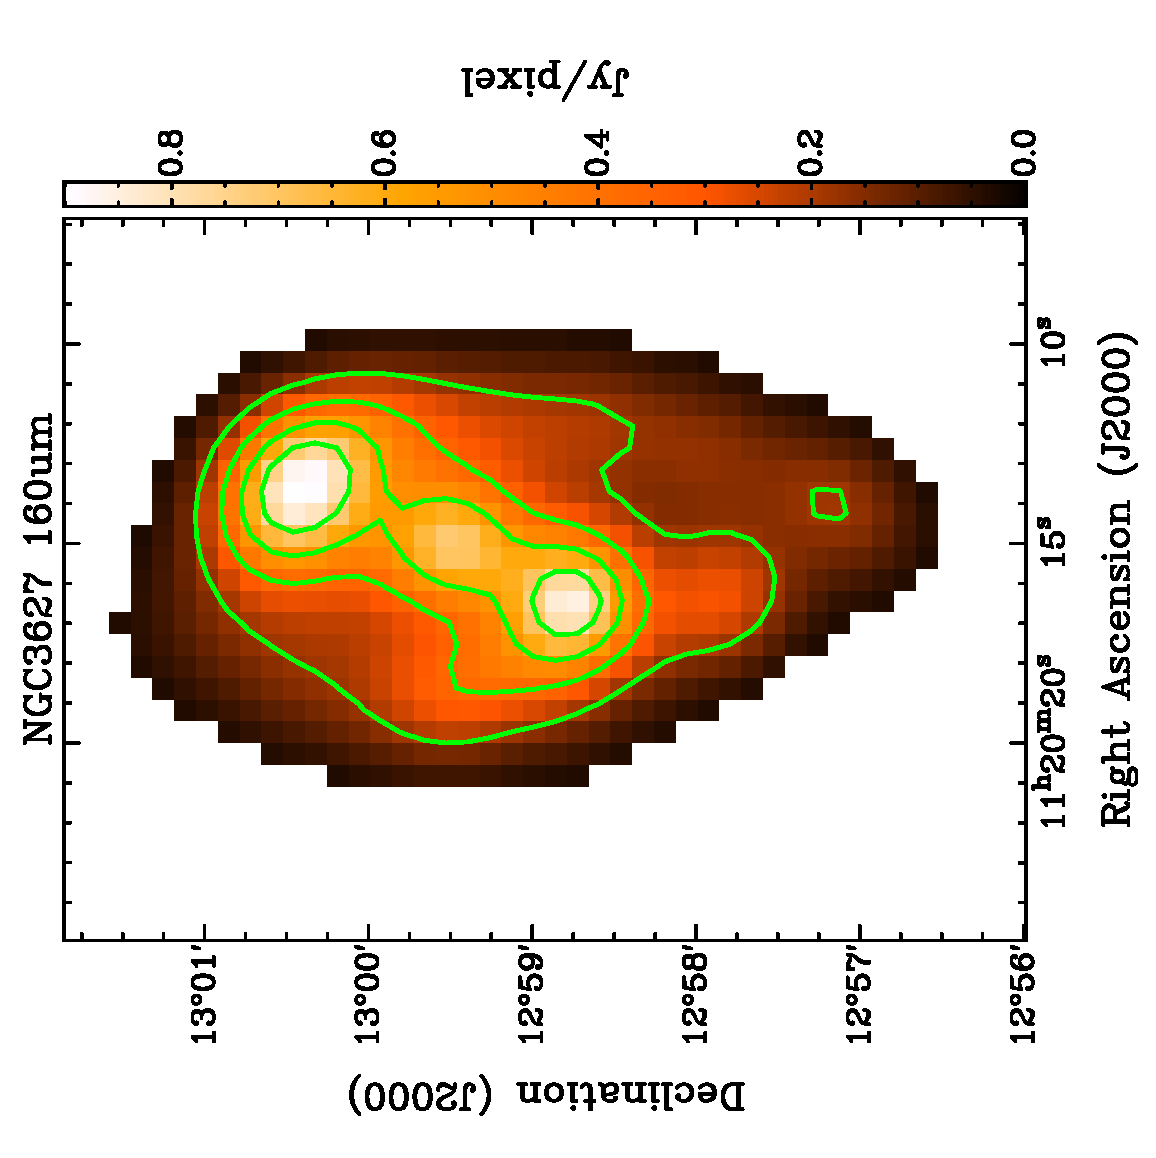
\includegraphics[width=1.\linewidth, angle=270]{sed_imgs/160_sed.eps}
%    \caption{160$\mu$m Observations}
  \end{subfigure}
  
  \begin{subfigure}[t]{0.48\textwidth}
    \centering
    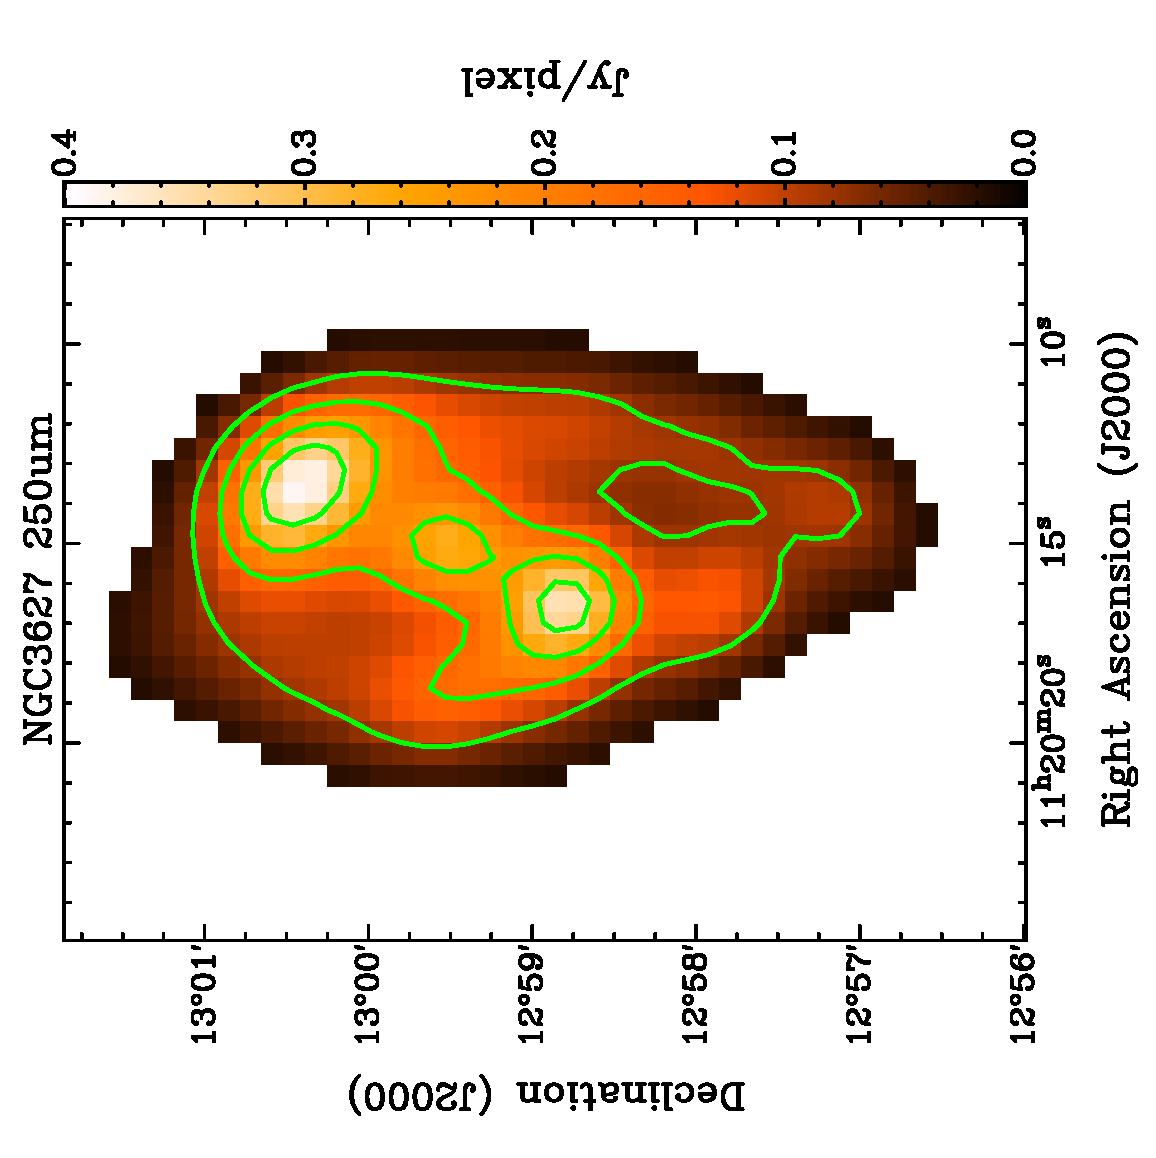
\includegraphics[width=1.\linewidth, angle=270]{sed_imgs/250_sed.eps}
%    \caption{250$\mu$m Observation}
  \end{subfigure}
  \quad
  \begin{subfigure}[t]{0.48\textwidth}
    \centering
    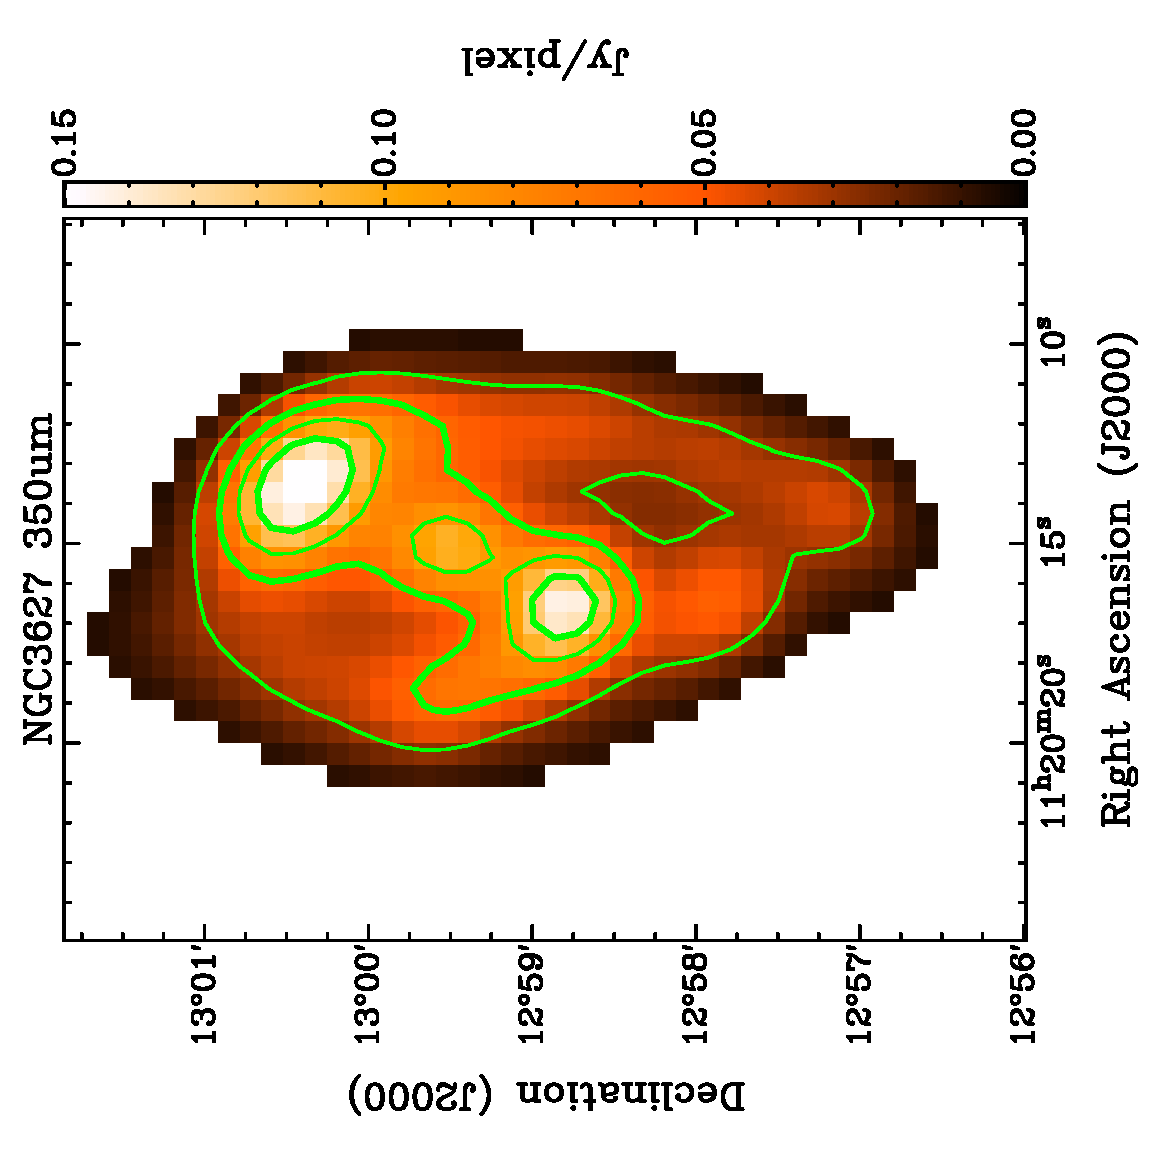
\includegraphics[width=1.\linewidth, angle=270]{sed_imgs/350_sed.eps}
%    \caption{350$\mu$m Observation}
  \end{subfigure}
  
  \caption[NGC3627 Observations Used in SED Fitting]{Observation of NGC3627 used for SED fitting.  Each of the images is on a 8$\arcsec$ by 8$\arcsec$ grid and has been convolved to 36.0$\arcsec$ with a 5$\sigma$ cut applied.  The contours for each image are 20\%, 40\%, 60\%, and 80\%.} 
  \label{fig:images}
\end{figure}  

\begin{figure}
  \ContinuedFloat 
  \begin{subfigure}[t]{0.48\textwidth}
    \centering
    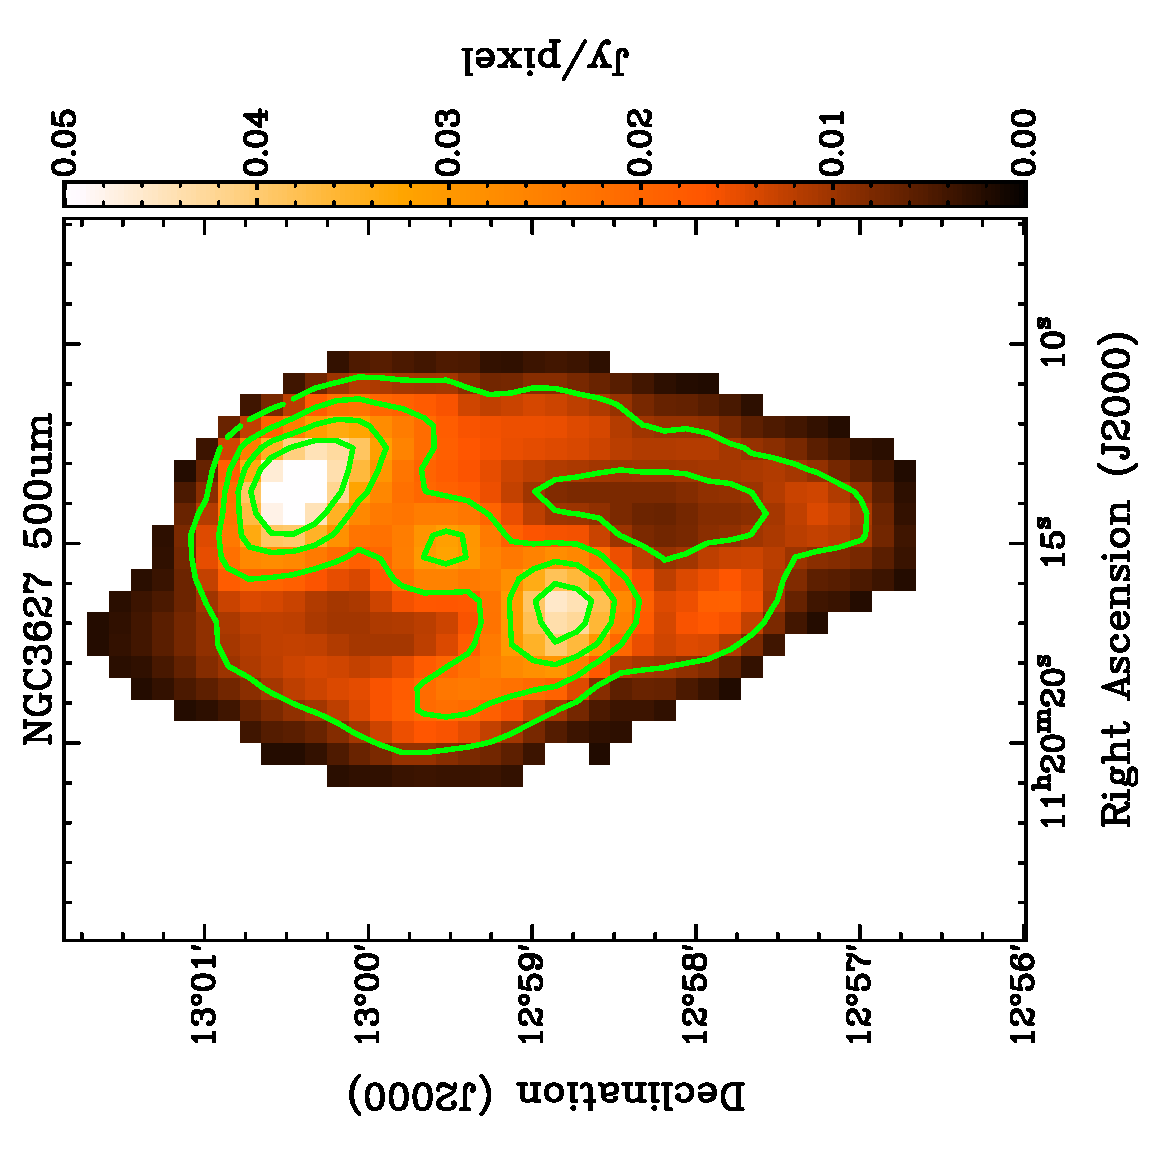
\includegraphics[width=1.\textwidth,angle=270]{sed_imgs/500_sed.eps}
  \end{subfigure}
  \quad
  \begin{subfigure}[t]{0.48\textwidth}
    \centering
    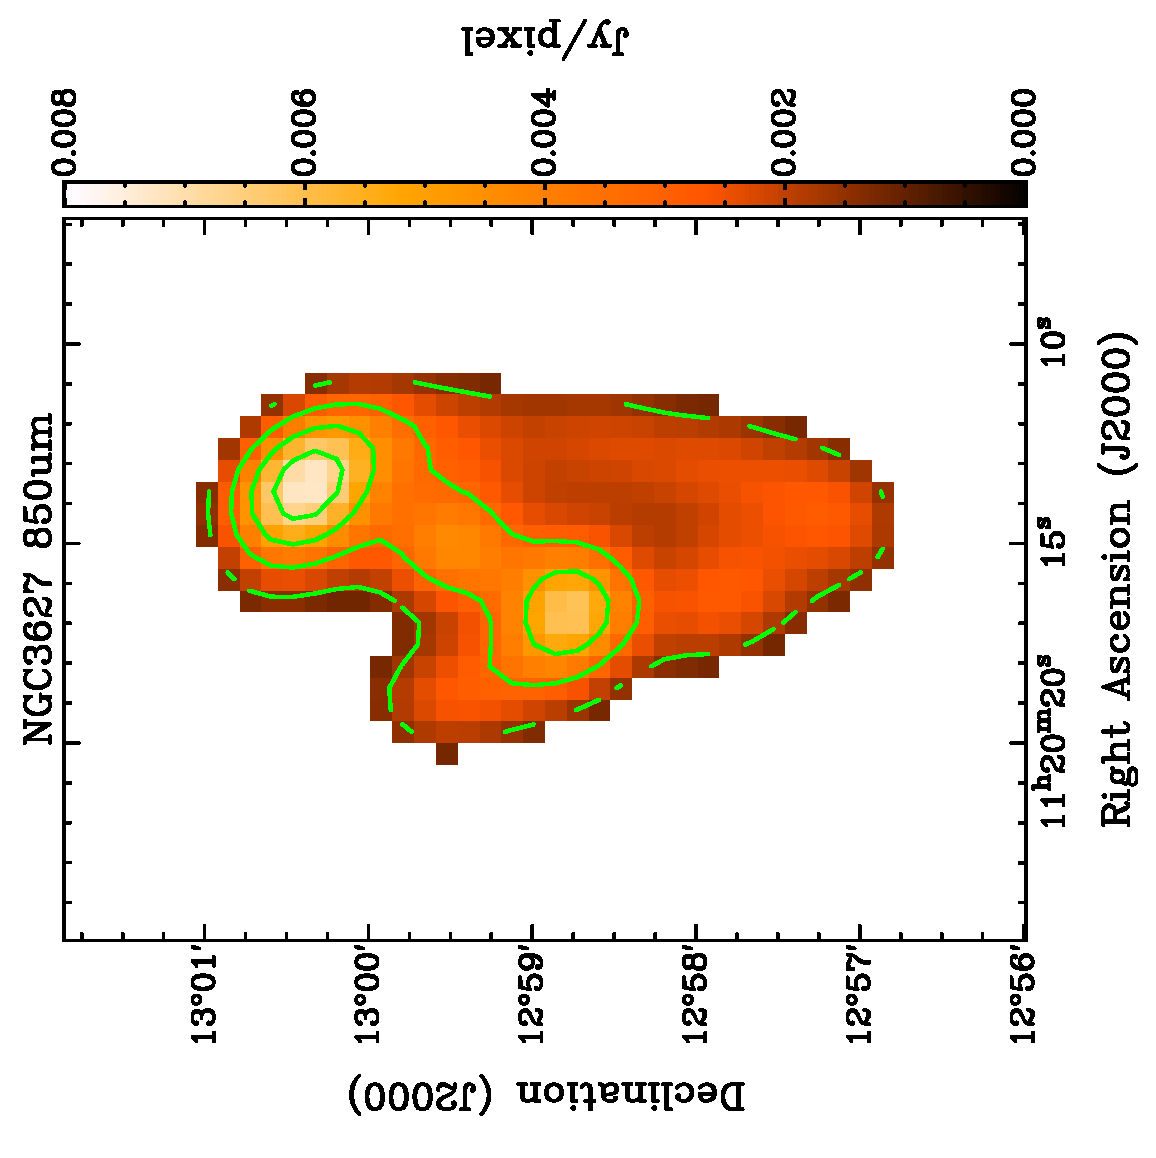
\includegraphics[width=1.\textwidth,angle=270]{sed_imgs/850_sed.eps}
  \end{subfigure}
  \caption{(continued)}
\end{figure}

The quality of the fit using the 450$\mu$m observations for the Li and Draine model of $\beta$=2 and $\kappa_{\nu,300}$=0.2665 is shown in Figure \ref{fig:w2_4}.  The quality of the fit is determined by how well the expected flux from the SED fitting matches the observed flux.  If the fits are able to recreate the observed emission, then all of the points will lie on the line $y=x$ shown in the plots as a black line.  If the SED is underestimating the flux, the points will appear below the 1 to 1 line, and an over estimation from the SED will result in points above the line.  

\begin{figure}
  \centering
  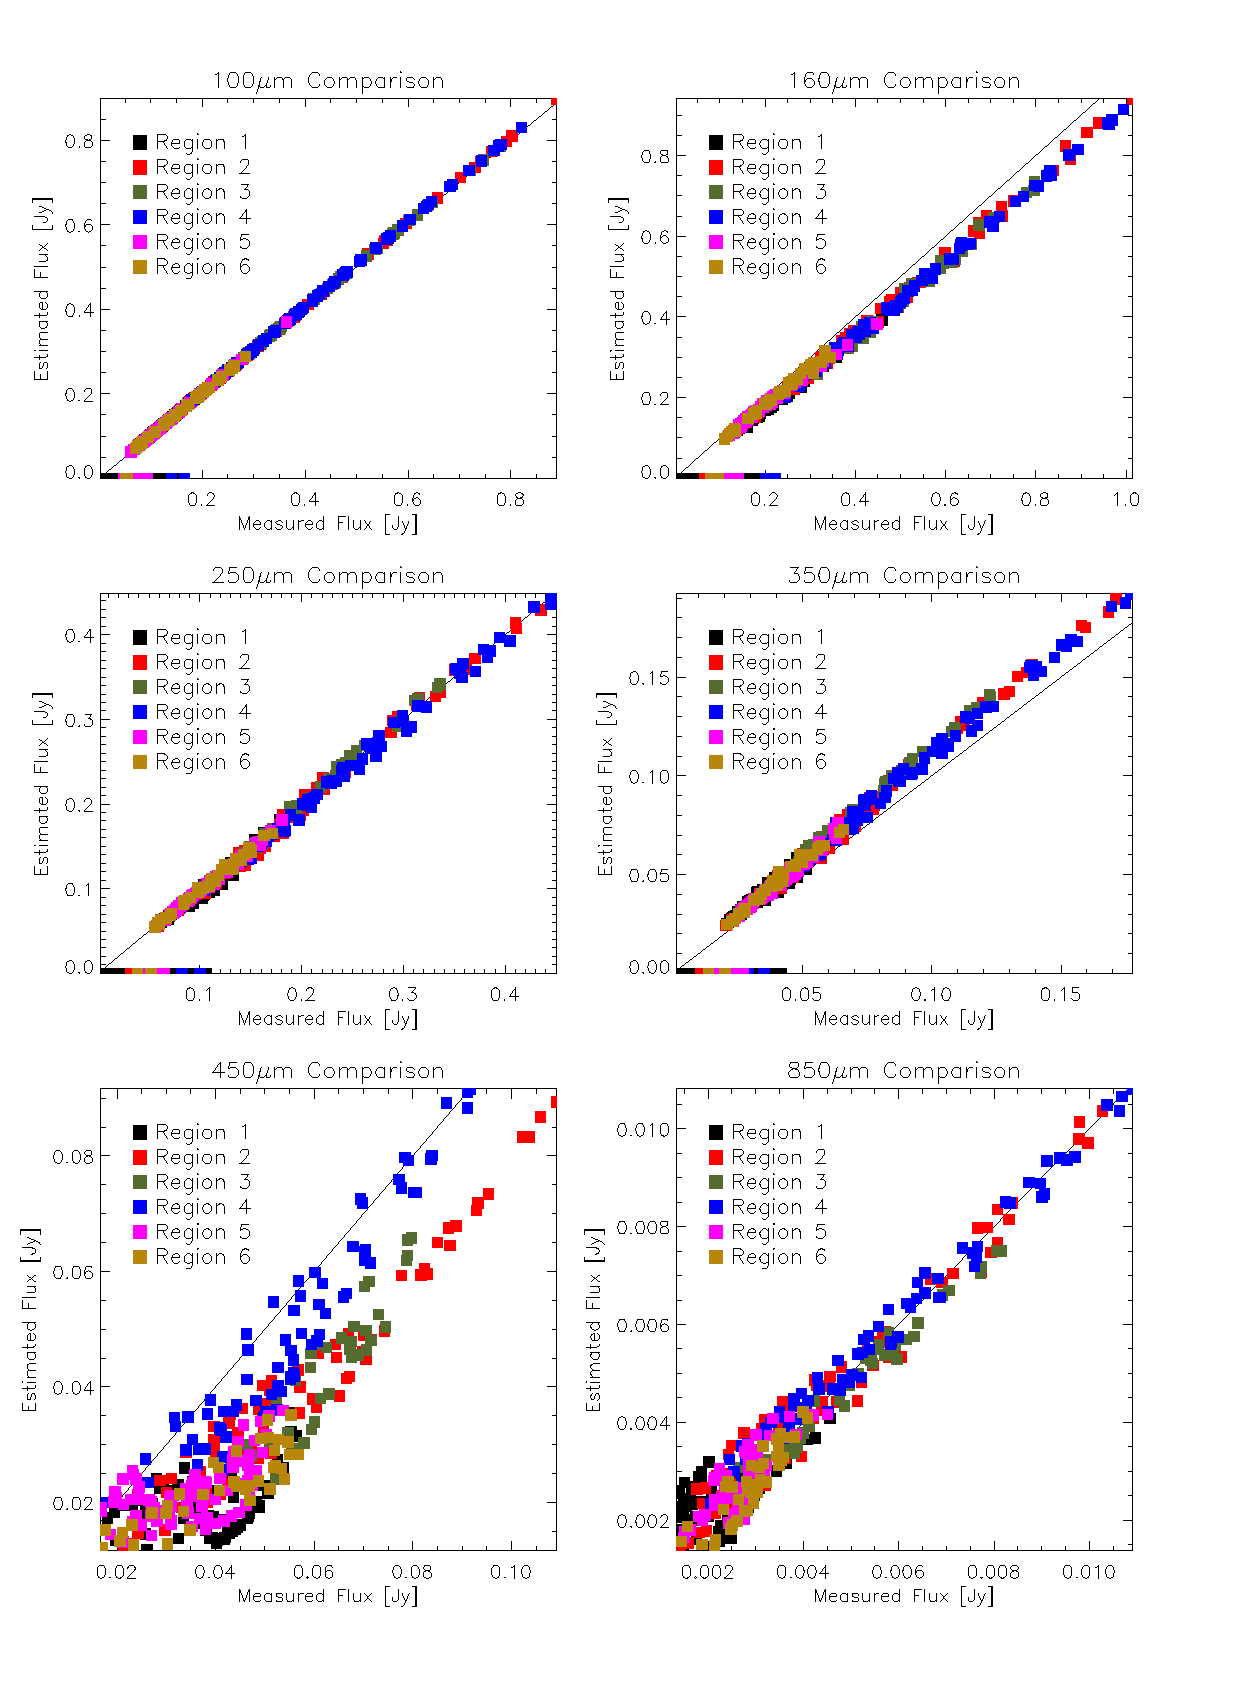
\includegraphics[width=1.\textwidth]{sed_imgs/flux_compare_2_4.eps}
  \caption[Li and Draine Model SED Fit Quality Using 450$\mu$m Data]{Quality of the SED fits to the Li and Draine model using the 450$\mu$m emission.  The regions shown are the regions in Figure \ref{fig:regions}.}
  \label{fig:w2_4}
\end{figure}

From Figure \ref{fig:w2_4}, the fitting procedure is able to handle the 100$\mu$m, 250$\mu$m, and 850$\mu$m with some slight under estimation in the 160$\mu$m and over  estimation in the 350$\mu$m.  The most compelling piece of information in Figure \ref{fig:w2_4} is the SED's inability to fit the observed 450$\mu$m flux despite the care taken to account for the odd beam shape of the 450$\mu$m data.  The discrepancy between the observed and fitted fluxes is not a result of a poor fit, but rather an intrinsic error in the 450$\mu$m observations.  The over abundance of flux present in the SCUBA-2 450$\mu$m data was determined to be an issue with the data itself rather than a signature of a physical process.  We determined that the 450$\mu$m data was overestimating the flux by calculating a 450$\mu$m flux using a linear fit between the filtered 350$\mu$m flux of 27.1 Jy and the filtered 500$\mu$m flux of 8.56 Jy.  The 450$\mu$m flux expected from these two data points was 14.7 Jy; however our 450$\mu$m flux was measured to be 20.6 Jy.

In order to avoid any errors in our final parameter maps, we substitute the 450$\mu$m emission with KINGFISH 500$\mu$m emission.  The quality of the fitted SEDs using the 500$\mu$m emission are shown in Figures \ref{fig:w1_5}, \ref{fig:w2_5}, and \ref{fig:wf_5} for the Planck model, Li and Draine model and the emissivity as a free parameter, respectively.  To assign a numerical quantity to the quality of the fit the vertical distance was calculated for each point to the 1 to 1 line and then summed.  The summed distances are shown in Table \ref{tab:lsq} and suggest the best fit comes from allowing the emissivity index to vary.  The resulting parameter maps of the fits using the 500$\mu$m observations are shown in Figure \ref{fig:param_fits}. The numerical values from fitting each model are shown in Tables \ref{tab:beta_1}, \ref{tab:beta_2}, and \ref{tab:beta_f} where each region corresponds to the regions labeled in Figure \ref{fig:regions}.

\begin{figure}
  \centering
  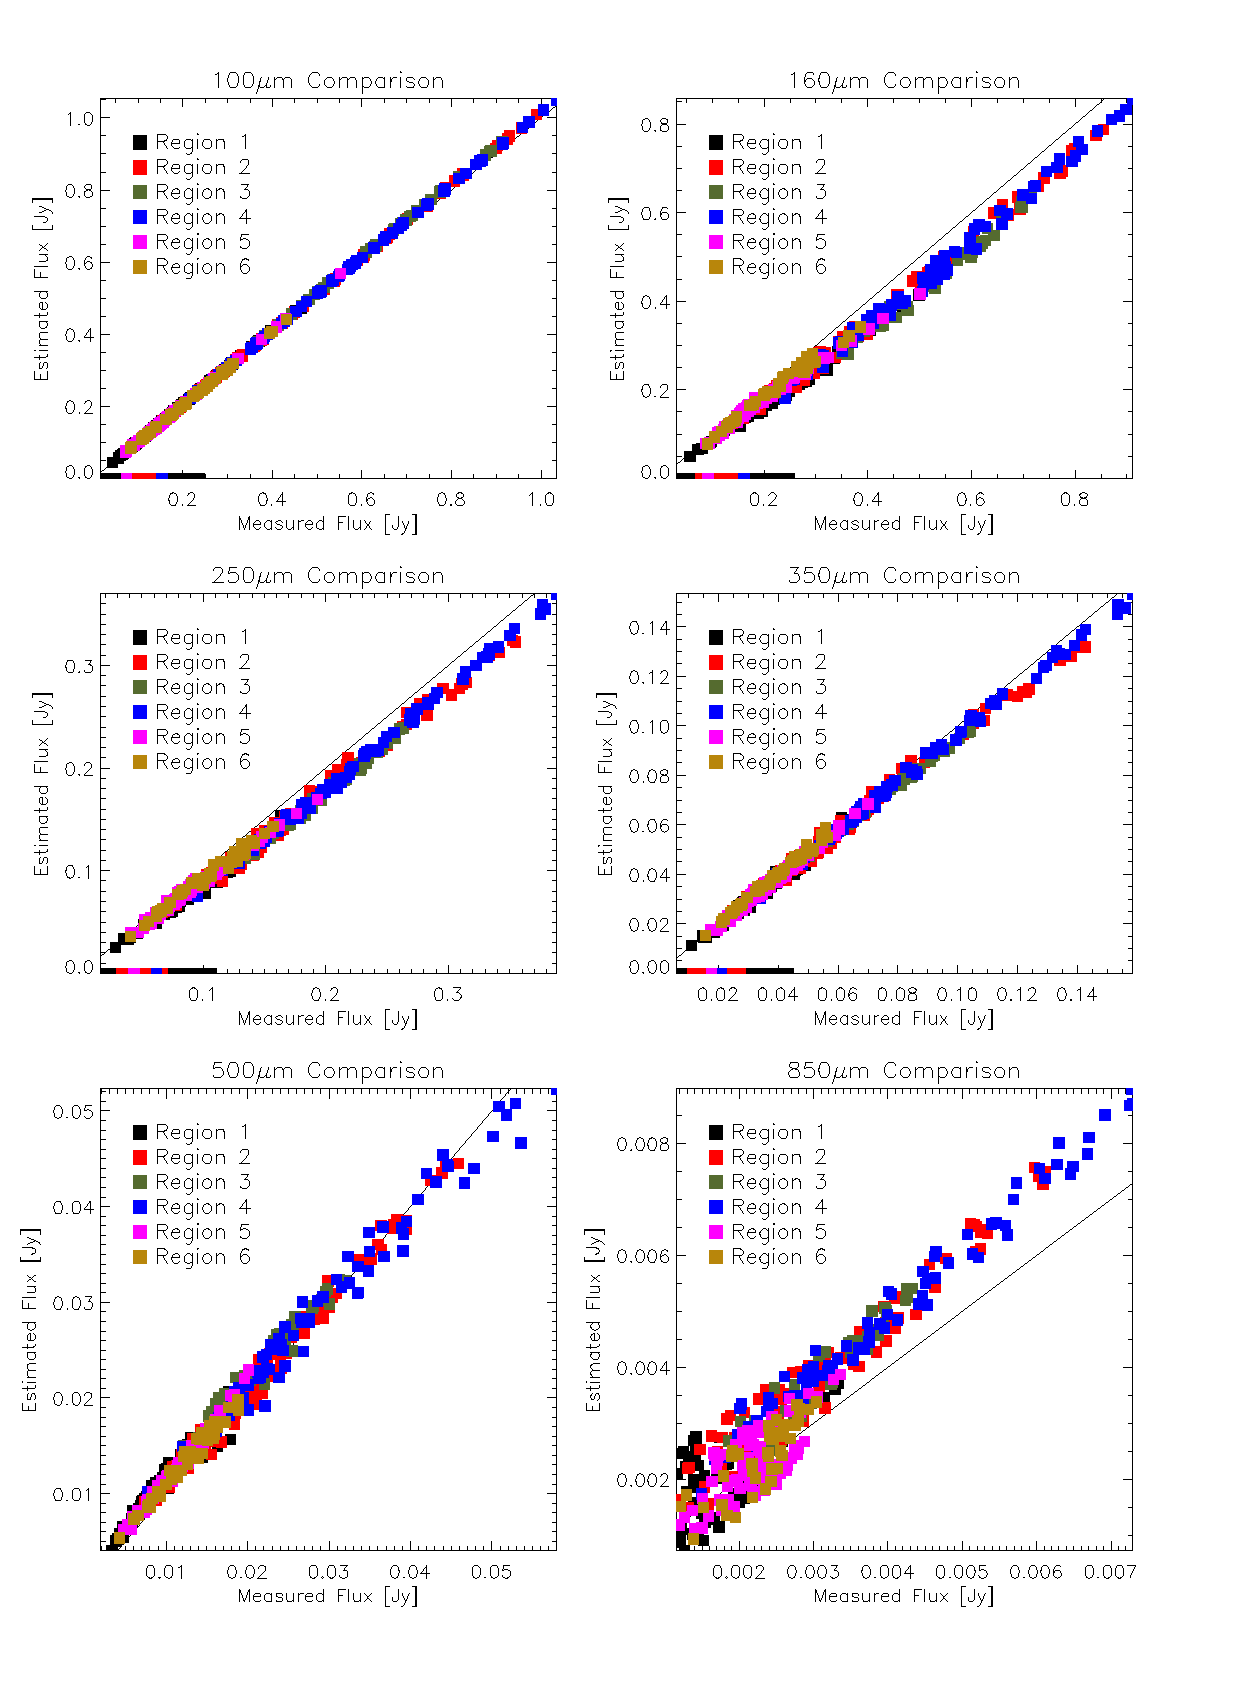
\includegraphics[width=1.\textwidth]{sed_imgs/flux_compare_1_5.eps}
  \caption[Planck Model SED Fit Quality Using 500$\mu$m Data]{Quality of the SED fits using the Planck model with the 500$\mu$m emission.  The regions shown are the regions in Figure \ref{fig:regions}.}
  \label{fig:w1_5}
\end{figure}

\begin{figure}
  \centering
  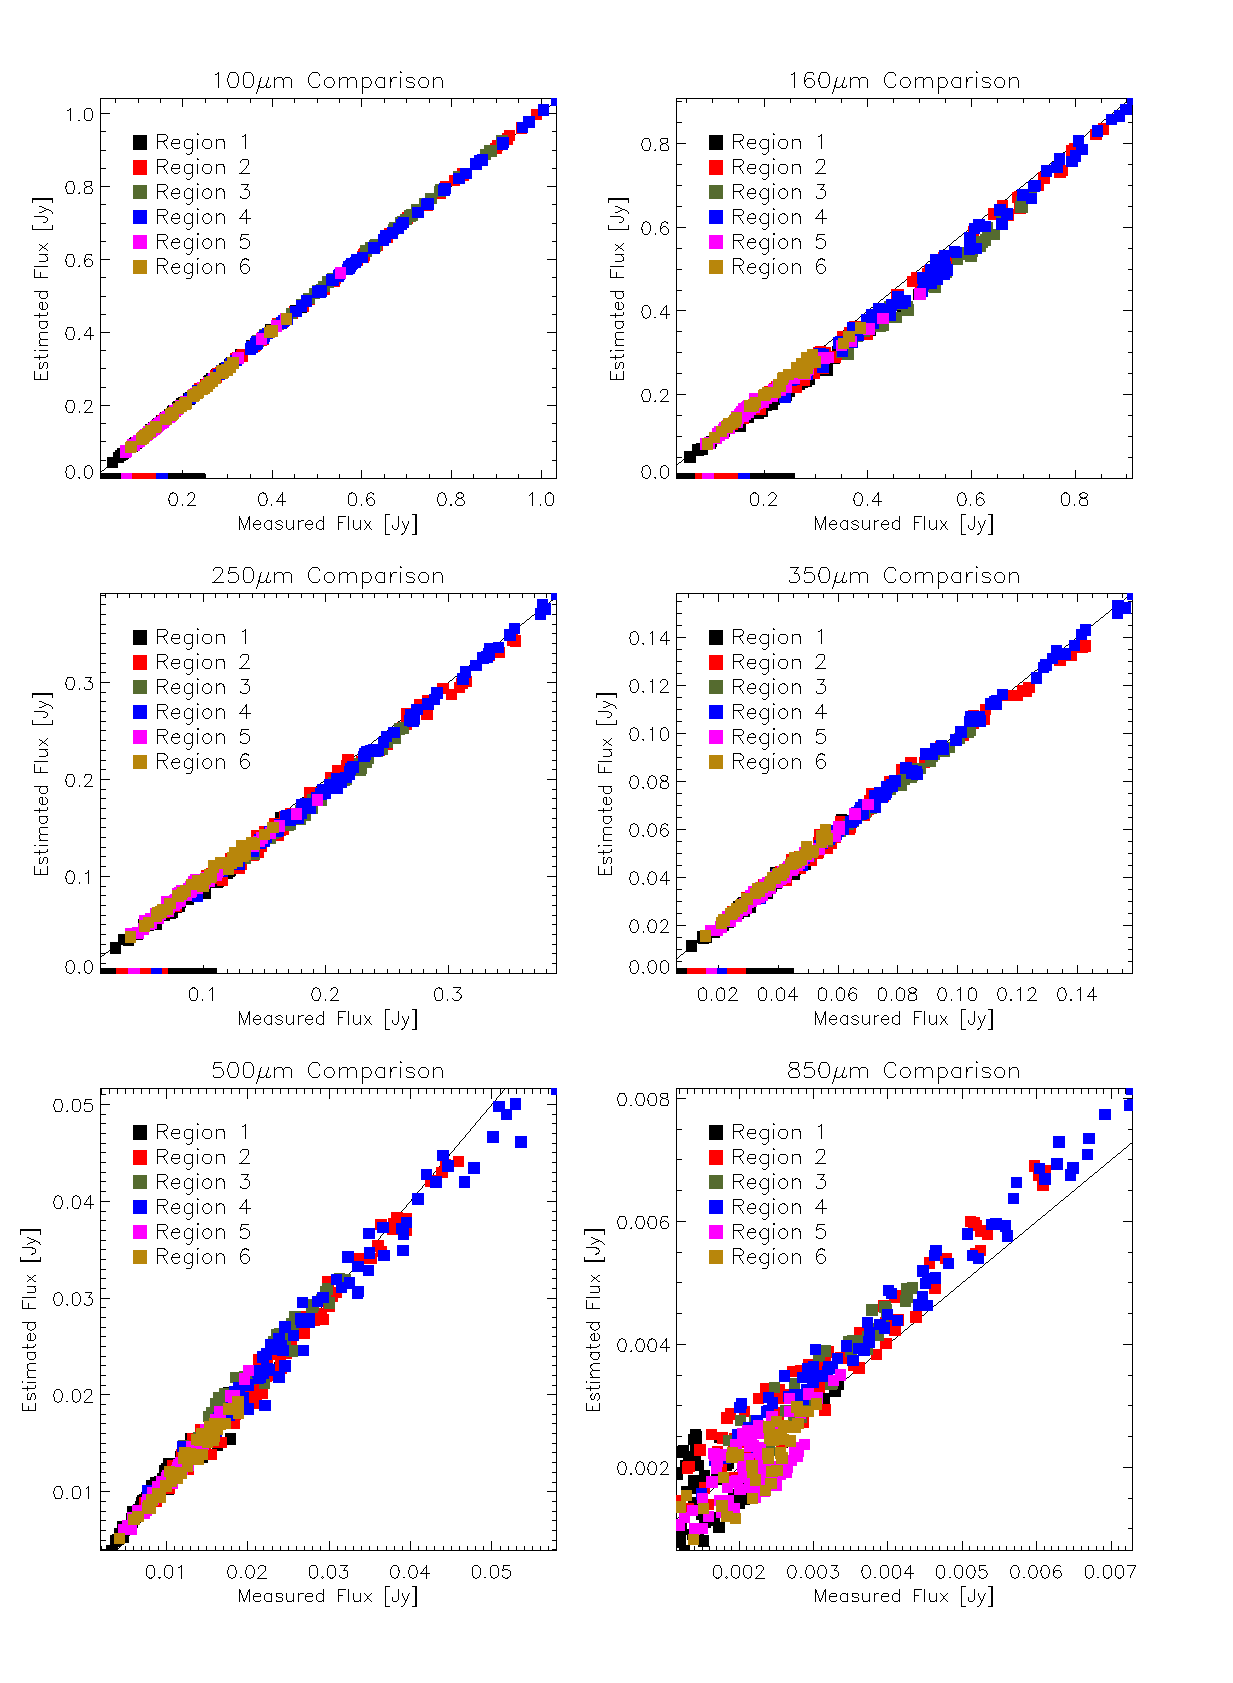
\includegraphics[width=1.\textwidth]{sed_imgs/flux_compare_2_5.eps}
  \caption[Li and Draine Model SED Fit Quality Using 500$\mu$m Data]{Quality of the SED fits using the Li and Draine model with the 500$\mu$m emission.  The regions shown are the regions in Figure \ref{fig:regions}.}
  \label{fig:w2_5}
\end{figure}

\begin{figure}
  \centering
  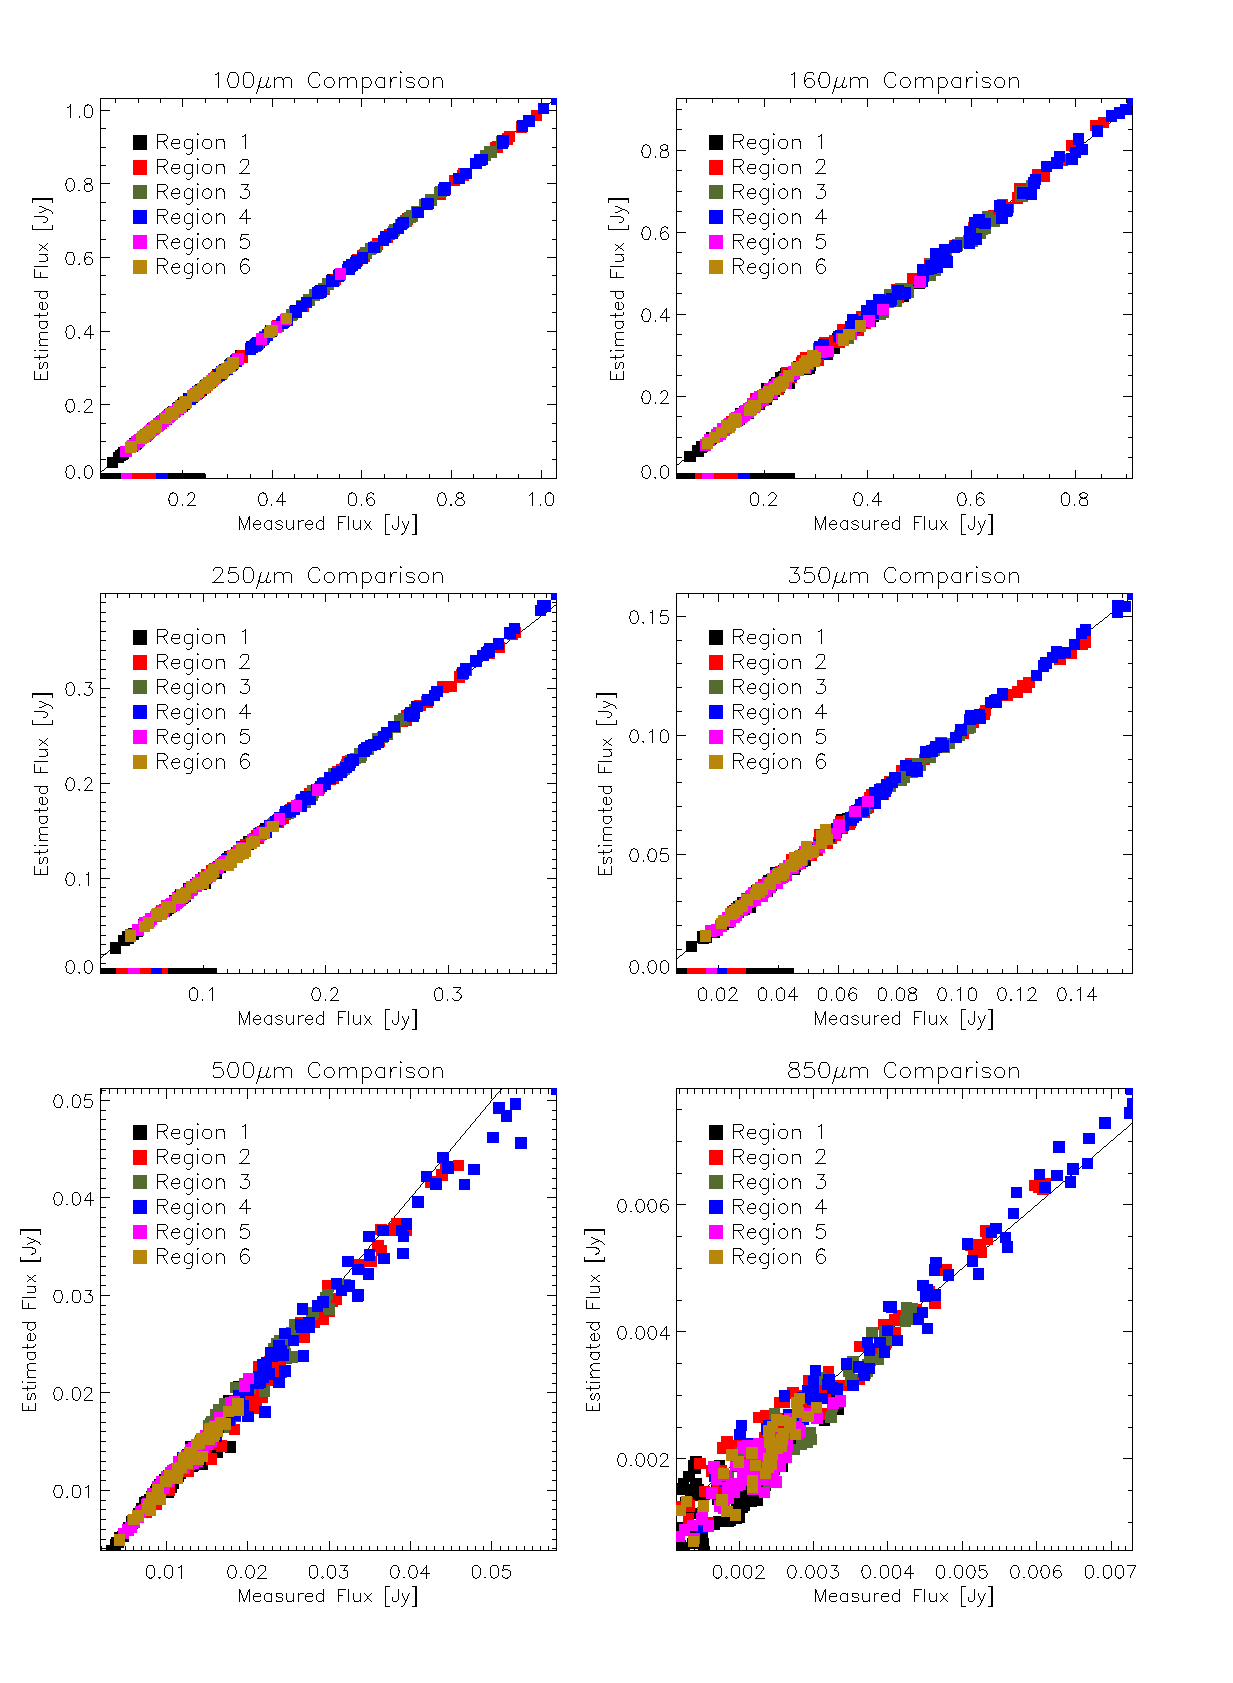
\includegraphics[width=1.\textwidth]{sed_imgs/flux_compare_free_5.eps}
  \caption[Emissivity as a Free Parameter SED Fit Quality using the 500$\mu$m Data]{Quality of the SED fits with the emissivity index as a free paramter with the 500$\mu$m emission.  The regions shown are the regions in Figure \ref{fig:regions}.}
  \label{fig:wf_5}
\end{figure}

\begin{deluxetable}{cccc}
  \tabletypesize{\footnotesize}
  \tablecolumns{4}
  \tablewidth{0pt}
  \tablecaption{Total Distance to 1 to 1 Line Using the 500$\mu$m Emission\label{tab:lsq}}
  \tablehead{\colhead{Observation} & \colhead{Planck Model} & \colhead{Li and Draine Model} & \colhead{Variable Emissivity Index} }
  \startdata
    100$\mu$m & 0.000    & 0.01245 & 0.1277  \\
    160$\mu$m & 15.55    & 8.979   & 2.159   \\
    250$\mu$m & 5.808    & 3.071   & 0.4465  \\ 
    350$\mu$m & 0.8045   & 0.3541  & 0.1161  \\
    500$\mu$m & 0.08192  & 0.1147  & 0.1866  \\
    850$\mu$m & 0.02825  & 0.05218 & 0.09528 \\
    Total     & 22.23    & 12.583  & 3.131   \\
  \enddata
\end{deluxetable}

\begin{deluxetable}{ccccc}
  \tabletypesize{\footnotesize}
  \tablecolumns{5}
  \tablewidth{0pt}
  \tablecaption{Best Fit Parameters for Planck Model Using 500$\mu$m Emission for Pixel Fits\label{tab:beta_1}}
  \tablehead{\colhead{Region} & \colhead{Average $\beta$} & \colhead{ Total Dust Mass} & \colhead{Average Dust} & \colhead{Average} \\ & &  $\left[10^5M_\odot\right]$ & Surface Density & Temperature \\ & & & $\left[M_\odot pc^{-2}\right]$ &[K]}
  \startdata
    1 & 1.8 & 52  $\pm$ 23 & 0.10 $\pm$ 0.05 & 26   $\pm$ 2   \\
    2 & 1.8 & 13  $\pm$ 4  & 0.12 $\pm$ 0.04 & 27   $\pm$ 1   \\
    3 & 1.8 & 6   $\pm$ 1  & 0.12 $\pm$ 0.02 & 28.8 $\pm$ 0.6 \\
    4 & 1.8 & 16  $\pm$ 6  & 0.15 $\pm$ 0.05 & 26   $\pm$ 1   \\
    5 & 1.8 & 10  $\pm$ 2  & 0.08 $\pm$ 0.02 & 24   $\pm$ 1   \\
    6 & 1.8 & 4   $\pm$ 1  & 0.08 $\pm$ 0.02 & 25   $\pm$ 1   \\
  \enddata
\end{deluxetable}

\begin{deluxetable}{ccccc}
  \tablecolumns{5}
  \tabletypesize{\footnotesize}
  \tablewidth{0pt}
  \tablecaption{Best Fit Parameters for Li and Draine Model Using 500$\mu$m Emission for Pixel Fits\label{tab:beta_2}}
  \tablehead{\colhead{Region} & \colhead{Average $\beta$} & \colhead{ Total Dust Mass} & \colhead{Average Dust} & \colhead{Average} \\ & &  $\left[10^5M_\odot\right]$ & Surface Density & Temperature \\ & & & $\left[M_\odot pc^{-2}\right]$ &[K]}
  \startdata
    1 & 2.0 & 230 $\pm$ 103 & 0.5  $\pm$ 0.2  & 24   $\pm$ 2   \\
    2 & 2.0 & 57  $\pm$ 19  & 0.6  $\pm$ 0.2  & 25   $\pm$ 1   \\
    3 & 2.0 & 28  $\pm$ 5   & 0.52 $\pm$ 0.09 & 26.4 $\pm$ 0.5 \\
    4 & 2.0 & 70  $\pm$ 22  & 0.7  $\pm$ 0.3  & 24.4 $\pm$ 0.8 \\
    5 & 2.0 & 42  $\pm$ 9   & 0.34 $\pm$ 0.08 & 22.4 $\pm$ 0.8 \\
    6 & 2.0 & 18  $\pm$ 4   & 0.33 $\pm$ 0.08 & 23.5 $\pm$ 0.9 \\
  \enddata
\end{deluxetable}

\begin{deluxetable}{ccccc}
  \tablecolumns{5}
  \tabletypesize{\footnotesize}
  \tablewidth{0pt}
  \tablecaption{Best Fit Parameters for $\beta$ As A Free Parameter Using 500$\mu$m Emission for Pixel Fits\label{tab:beta_f}}
  \tablehead{\colhead{Region} & \colhead{Average $\beta$} & \colhead{ Total Dust Mass} & \colhead{Average Dust} & \colhead{Average} \\ & &  $\left[10^5M_\odot\right]$ & Surface Density & Temperature \\ & & & $\left[M_\odot pc^{-2}\right]$ &[K]}
  \startdata
    1 & 2.2  $\pm$ 0.2  & 73 $\pm$ 31 & 0.14 $\pm$ 0.06 & 22   $\pm$ 1   \\
    2 & 2.3  $\pm$ 0.2  & 18 $\pm$ 5  & 0.18 $\pm$ 0.05 & 22   $\pm$ 2   \\
    3 & 2.34 $\pm$ 0.09 & 9  $\pm$ 1  & 0.18 $\pm$ 0.02 & 23.0 $\pm$ 0.9 \\
    4 & 2.2  $\pm$ 0.1  & 22 $\pm$ 5  & 0.21 $\pm$ 0.05 & 22   $\pm$ 1   \\
    5 & 2.1  $\pm$ 0.2  & 12 $\pm$ 4  & 0.10 $\pm$ 0.03 & 22   $\pm$ 1   \\
    6 & 2.1  $\pm$ 0.1  & 5  $\pm$ 1  & 0.09 $\pm$ 0.03 & 23.0 $\pm$ 0.9 \\
  \enddata
\end{deluxetable}

\begin{figure}
  \centering
  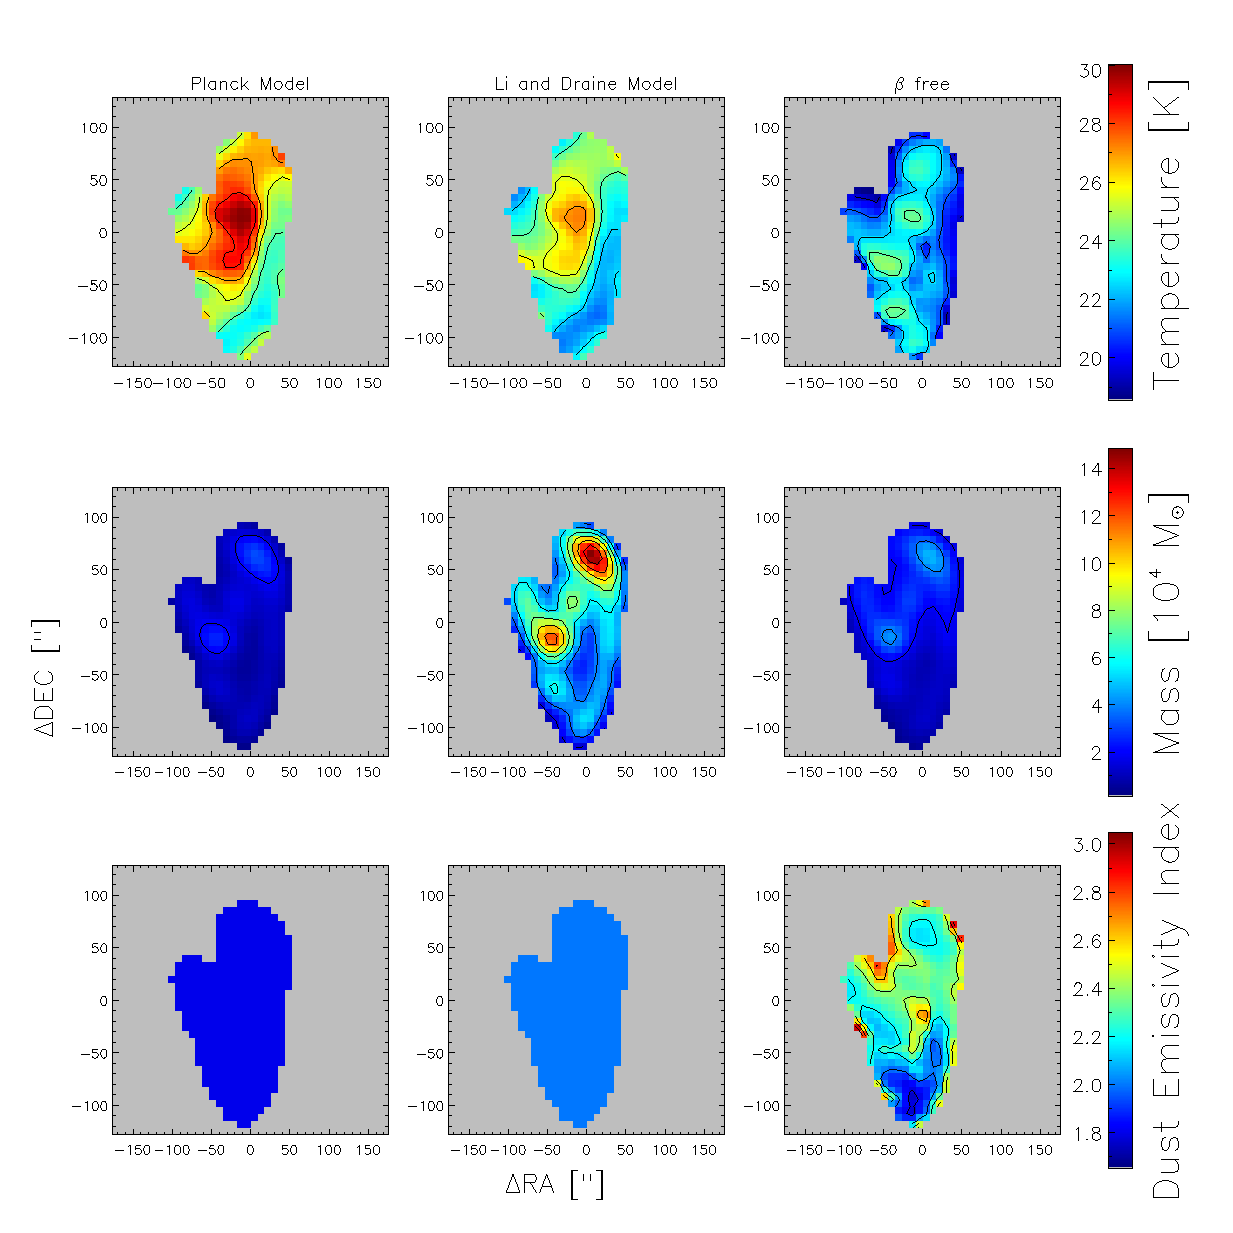
\includegraphics[width=1.\textwidth]{sed_imgs/parameter_full.eps}
  \caption[SED Parameter Maps]{Returned value for the SED fits using the 500$\mu$m observations with the Planck model in the left column, the Li and Draine model in the middle column, and $\beta$ as a free variable in the right column.  The top row shows the temperature with contours from 19.5K to 28.5K in 1.5K increments.  The second row show the returned masses with contours from 1.9M$_\odot$ to 13.3M$_\odot$ in 1.9M$_\odot$ increments.  The Li and Draine mass fits have been divided by three to better show the features relative to the other two fits.  The bottom row shows the returned dust emissivity index values with contours from 1.8 to 2.8 with 0.2 increments.}
  \label{fig:param_fits}
\end{figure}

\subsection{Total Region Flux SED Fits}

The second method used to determine the dust mass was to fit the SED to the flux of each region in Figure \ref{fig:regions}.  Performing the fit in this manner is beneficial because it increases the signal to noise of the region and produces a more precise set of parameters.  Initially, fitting the total flux of each region was carried out in the same manner as the individual pixel fits by fixing the emissivity index to 1.8 and 2.0, and allowing the emissivity index to vary.  This method ran into issues when determining an initial mass to use in the fitting.  If we used the same procedure as we did for the pixel fitting, equation \ref{eq:mass}, our initial masses would either converge on a local minimum or not be able to produce a useable fit.  This was due to the Levenberg-Marquardt method not being able to efficiently step through the parameter space to find a useable minimum, or the method would converge to a local minimum instead of the global minimum.  The behavior of the fitted parameters with respect to the initial mass is shown in Figure \ref{fig:init_mass_bf} for a variable emissivity index.  

In order to prevent any false convergences, we established a range of emissivity index values from 1.6 to 2.9 with increments of 0.05 and found the best fit mass and temperature for each of these indices.  This method ended up being significantly more robust than allowing the emissivity index to vary.  The relationship between the initial mass and the fitted parameters with a fixed emissivity is shown in Figure \ref{fig:init_mass_b1}, and shows the results are independent of the initial mass up to a cutoff point where the Levinberg-Marquardt method is unable to produce reliable fits.  Determining the best emissivity index was decided by which value returned the lowest reduced $\chi^2$ value.  The reduced $\chi^2$ and emissivity index plots are shown in Figure \ref{fig:beta_reg_sel} for each of the regions of NGC3627, where the minimum value is marked by the red line.  The best fit results using this method are shown in Table \ref{tab:region_vals} using the opacity suggested by the Planck model and the fitted SEDs are shown in Figure \ref{fig:SED_region}.

\begin{figure}
  \centering
  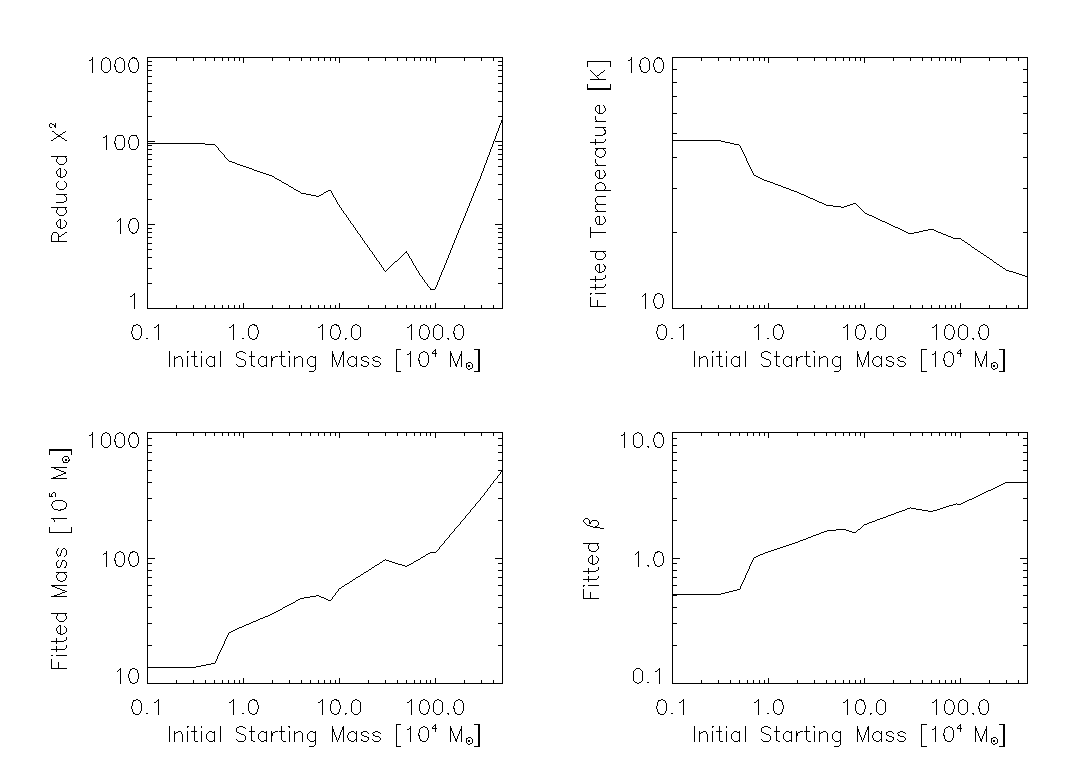
\includegraphics[width=1.\textwidth]{sed_imgs/beta_f_return.eps}
  \caption[Initial Mass Dependence and Convergence of SED Fits for Region Fluxes and Variable Emissivity Index]{Returned SED fitting output for region 1 with Planck opacity for the $\chi^2$, temperature, mass, and emissivity index with varying initial mass.  The top left panels shows the $\chi^2$ values for each starting mass.  The top right, bottom left, and bottom right panel show the returned temperatures, mass, and emissivity index.}
  \label{fig:init_mass_bf}
\end{figure}

\begin{figure}
  \centering
  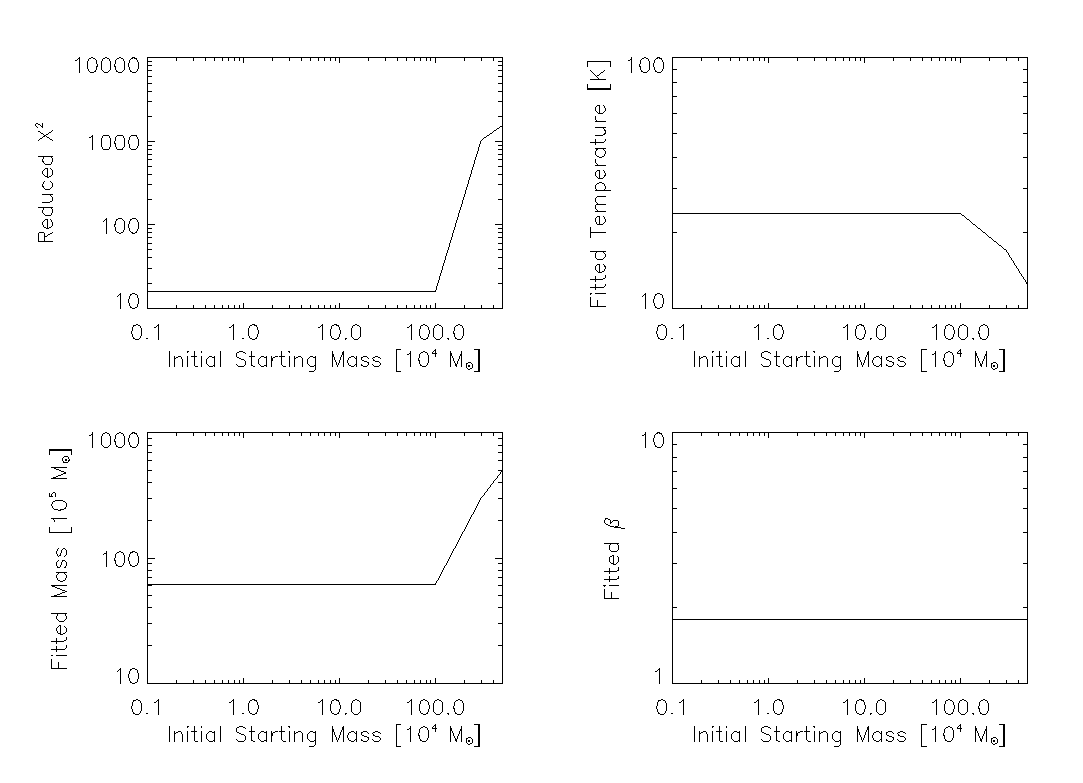
\includegraphics[width=1.\textwidth]{sed_imgs/beta_1_return.eps}
  \caption[Initial Mass Dependence and Convergence of SED Fits for Region Fluxes and Fixed Emissivity Index]{The same as Figure \ref{fig:init_mass_bf}, however the emissivity index has been fixed to 1.8.}
  \label{fig:init_mass_b1}
\end{figure}

\begin{figure}
  \centering
  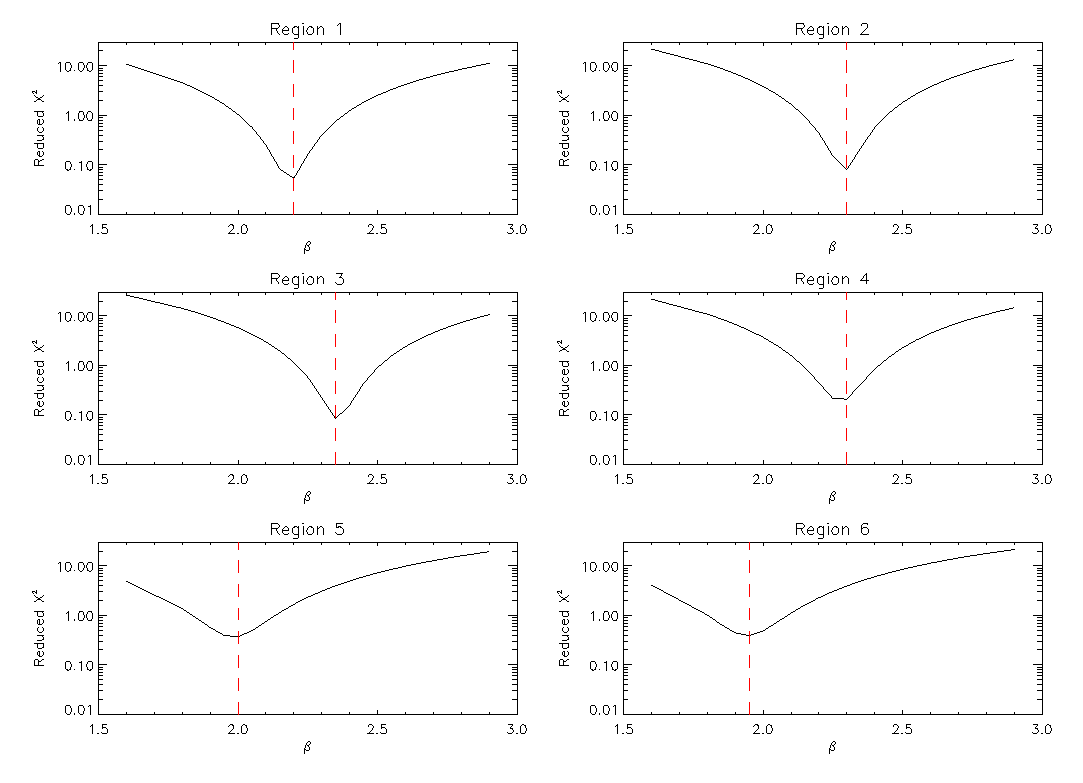
\includegraphics[width=1.\textwidth]{sed_imgs/beta_vals.eps}
  \caption[Region Flux Best Emissivity Index Selection]{Plots for each region from figure \ref{fig:regions} showing the Fixed emissivity index value and the resulting reduced $\chi^2$ value.}
  \label{fig:beta_reg_sel}
\end{figure}

\begin{deluxetable}{ccccc}
  \tablecolumns{5}
  \tablewidth{0pt}
  \tablecaption{Best Fit Parameters for Planck Opacity Using Region Fluxes\label{tab:region_vals}}
  \tabletypesize{\footnotesize}
  \tablehead{\colhead{Region} & \colhead{Average $\beta$} & \colhead{Dust Mass} & \colhead{Average Dust} & \colhead{Temperature} \\ & &  $\left[10^5M_\odot\right]$ & Surface Density & [K]\\ & & & $\left[M_\odot pc^{-2}\right]$ &}
  \startdata
    1 & 2.20 $\pm$ 0.03 & 70   $\pm$ 5   & 0.14  $\pm$ 0.01  & 22.8 $\pm$ 0.5 \\
    2 & 2.30 $\pm$ 0.03 & 19   $\pm$ 1   & 0.18  $\pm$ 0.01  & 22.5 $\pm$ 0.3 \\
    3 & 2.35 $\pm$ 0.03 & 9.5  $\pm$ 0.6 & 0.21  $\pm$ 0.01  & 23.3 $\pm$ 0.3 \\
    4 & 2.30 $\pm$ 0.03 & 23   $\pm$ 1   & 0.22  $\pm$ 0.01  & 22.2 $\pm$ 0.2\\
    5 & 2.00 $\pm$ 0.03 & 11.4 $\pm$ 0.8 & 0.093 $\pm$ 0.007 & 22.3 $\pm$ 0.4\\
    6 & 1.95 $\pm$ 0.03 & 4.6  $\pm$ 0.3 & 0.087 $\pm$ 0.006 & 23.9 $\pm$ 0.4 \\
  \enddata
\end{deluxetable}

%it might be better to make this one figure with multiple SED's on it
\begin{figure}
  \centering
  \begin{subfigure}[t]{1\textwidth}
    \centering
    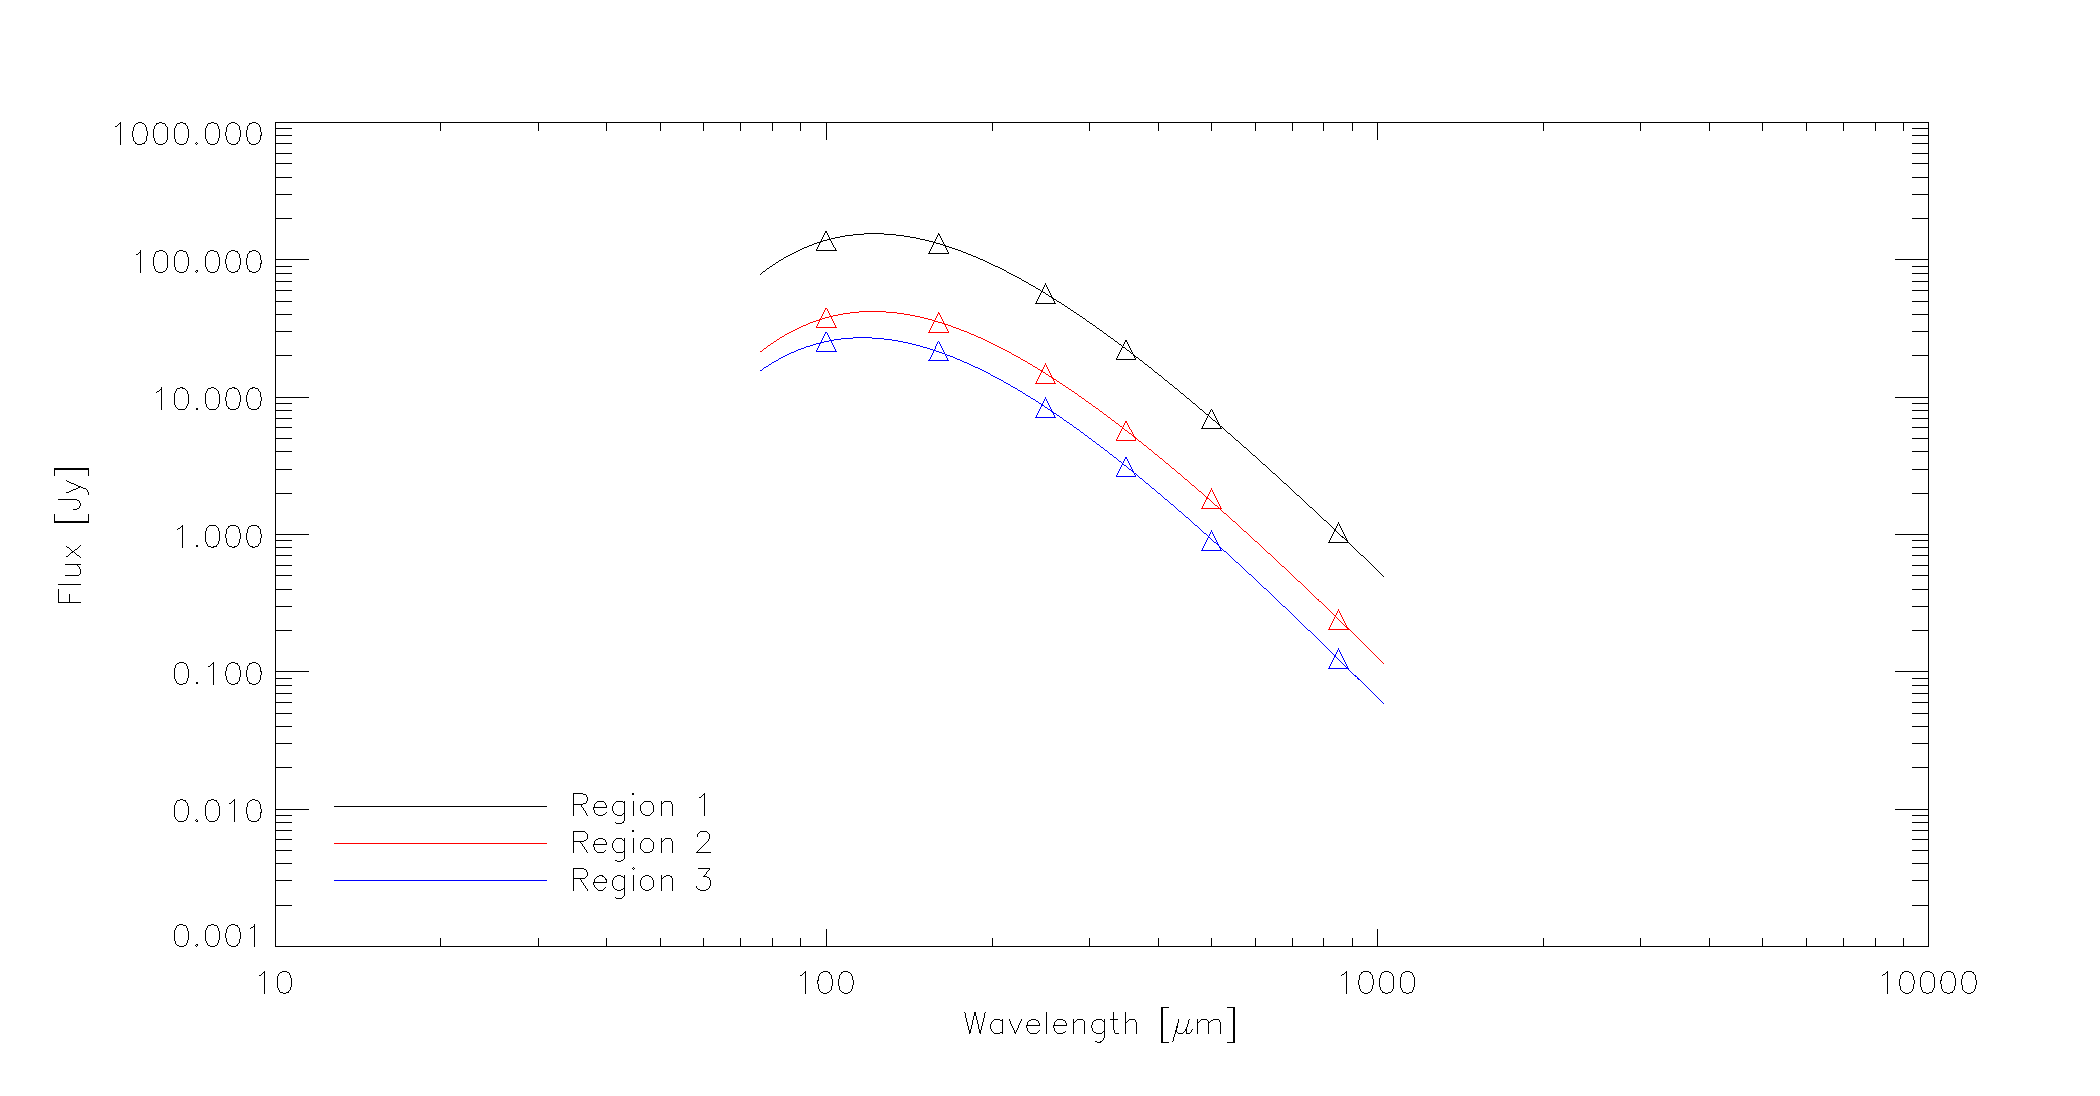
\includegraphics[width=1\linewidth]{sed_imgs/123.eps}
    \caption{Regions 1, 2, and 3 SEDs}
  \end{subfigure}
  
  \begin{subfigure}[t]{1\textwidth}
    \centering
    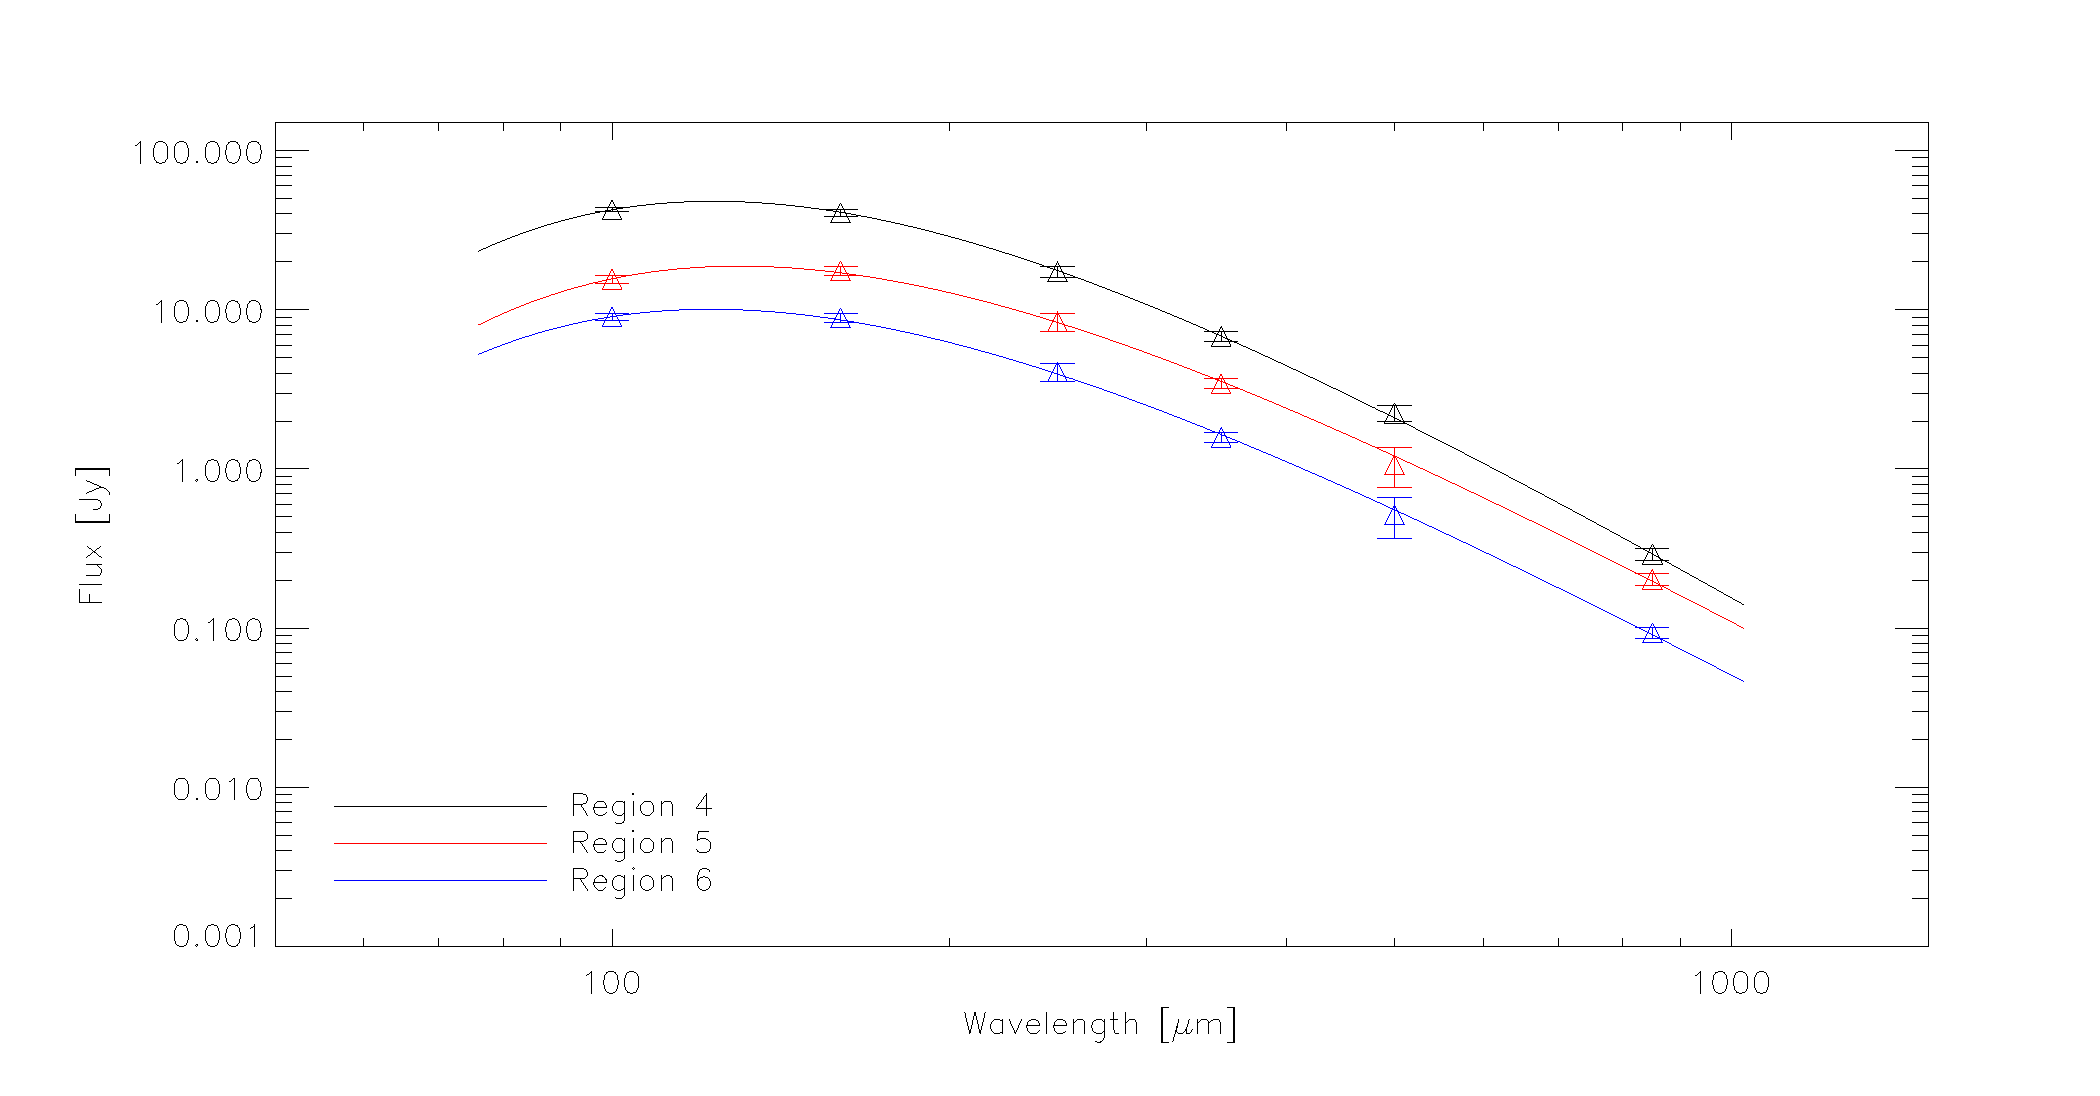
\includegraphics[width=1.\linewidth]{sed_imgs/456.eps}
    \caption{Regions 4, 5, and 6 SEDs}
  \end{subfigure}
  \caption[Region Flux SED Fits]{SED fits for the flux of each region in Figure \ref{fig:regions} using the Planck Opacity and allowing the emissivity index, $\beta$ to vary.}
  \label{fig:SED_region}
\end{figure}
  
\section{Discussion}
\subsection{Reliability of Individual Pixel Fits}

The issue of whether or not the individual pixel fits are reliable for a variable emissivity index is raised after seeing a strong dependence with the initial mass of the region SED fits shown in Figure \ref{fig:init_mass_bf}.  The argument can be made that since both fits have returned the same temperature (T$_{pixel}$=22$\pm$1 K and T$_{region}$=22.8$\pm$0.5 K), emissivity index ($\beta_{pixel}$=2.2$\pm$0.2 and $\beta_{region}$=2.20$\pm$0.03), and mass (M$_{pixel}$=85$\pm$38 M$_\odot$ and M$_{region}$=82$\pm$6 M$_\odot$), after the removal of any initial mass dependence for the region fits, the initial values for the pixel fits are able to locate the global minimum of the $\chi^2$ space regardless of any dependence.  The inability of the region fits to successfully converge was due to an overestimate of the initial mass, and was shown by the fitting routine returning the input parameters or the returned values would vary significantly given minor changes to the starting mass.  The mass associated with the 250$\mu$m flux using the 20 K Li and Draine model was scaling the peak of the SED to values larger than what would be expected using the Planck model which is the opacity used for the region fits.  The difference between the two initial masses was large enough for the Levenberg-Marquardt method to fail at finding a minimum.  This could be remedied by retooling the initial mass to use the Planck model; however by cycling through emissivity index values, we have provided a more reliable check to our pixel maps by breaking the dependency with the initial mass.

\subsection{Comparison with Previous Work}

We can check the validity of our results by comparing them to previous SED fits using the KINGFISH data \citep{galametz2012}.  Their best fit parameters were T=20.2K$\pm$1.4K and $\beta$=2.3$\pm$0.2 which agree within the uncertainties with our results of T=22K$\pm$1K and $\beta$=2.2$\pm$0.2 for a variable emissivity index.  However, the dust mass reported by \cite{galametz2012} was 7.82$^{+0.80}_{-0.66}\times$10$^7$ M$_\odot$ using the opacity model from Li and Draine, and our reported dust mass for the region fits was 7.0$\pm$0.5$\times$10$^6$ M$_\odot$ using the Planck opacity.  To check the agreement between our mass and that of \cite{galametz2012} we need to take into account several differences in the two analyses. The differences consist of a lower flux from the extended structure removal in our data set, the opacity values used, which wavelength was used to calculate the mass, and finally how an increase or decrease in the temperature or emissivity index can affect the mass.  

If we use the equation for mass given in \cite{parkin2012} for Centaurus A, we can extract the distance from the constant to get 

\begin{equation}\label{eq:mass_test}
  M=364\,D^{2}_{Mpc}S_{250\mu m}\left(e^{57.58 / T} - 1\right)
\end{equation}

\noindent We use equation \ref{eq:mass_test} for a simple comparison of our fit with that of \cite{galametz2012} based on only the temperature and observed flux at 250$\mu$m.  With our regional flux, we get a mass of 2.29$\times$10$^{7}$ M$_\odot$ using our temperature of 22 K and S$_{250\mu m}$=56 Jy from the sum of the 250$\mu$m pixels used to generate the maps shown in Figure \ref{fig:param_fits}.  Using the temperature of 20 K and S$_{250\mu m}$ = 96.7 Jy from \cite{galametz2012} gives a mass of 5.22$\times$10$^7$ M$_\odot$.  The disagreement in the masses can be partly attributed to the difference in temperatures; however, this will only decrease the mass calculated using the values from \cite{galametz2012} by 25\% which still leaves their mass higher than our mass.  The lower mass can also be attributed to our lower fluxes which are due to the extended emission removal and any calibration differences between the two data sets as well as any corrections that were applied in \cite{galametz2012} to calculate their flux.  The difference in fluxes will decrease the mass using the information from \cite{galametz2012} by another 42\%, bringing the two masses into agreement.

\subsection{Effects of 850$\mu$m Emission}

The major difference between our work on NGC3627 and the work done in \cite{galametz2012} is the presence of the 850$\mu$m data point.  We tested the effect of the 850$\mu$m data by excluding it from our fits.  The returned values for a variable emissivity index are shown in Table \ref{tab:no_850}.  The presence of the 850$\mu$m has little effect on the returned parameters.  

\begin{deluxetable}{ccccc}
  \tablecolumns{5}
  \tablewidth{0pt}
  \tablecaption{Best Fit Parameters Excluding 850$\mu$m Emission Using Planck Opacity with Variable Emissivity Index\label{tab:no_850}}
  \tabletypesize{\footnotesize}
  \tablehead{\colhead{Region} & \colhead{Average $\beta$} & \colhead{Dust Mass} & \colhead{Average Dust} & \colhead{Temperature} \\ & &  $\left[10^5M_\odot\right]$ & Surface Density & [K]\\ & & & $\left[M_\odot pc^{-2}\right]$ &}
  \startdata
    1 & 2.3 $\pm$ 0.3 & 75 $\pm$ 28 & 0.15 $\pm$ 0.06 & 22 $\pm$ 2 \\
    2 & 2.3 $\pm$ 0.3 & 18 $\pm$ 5  & 0.17 $\pm$ 0.05 & 23 $\pm$ 2 \\
    3 & 2.4 $\pm$ 0.2 & 10 $\pm$ 1  & 0.19 $\pm$ 0.02 & 23 $\pm$ 1 \\
    4 & 2.2 $\pm$ 0.2 & 22 $\pm$ 5  & 0.21 $\pm$ 0.05 & 23 $\pm$ 2 \\
    5 & 2.3 $\pm$ 0.2 & 14 $\pm$ 3  & 0.11 $\pm$ 0.03 & 21 $\pm$ 1 \\
    6 & 2.2 $\pm$ 0.2 &  5 $\pm$ 1  & 0.10 $\pm$ 0.02 & 22 $\pm$ 1 \\
  \enddata
\end{deluxetable}

The absence of a significant change in the returned parameters indicates a lack of any excess submillimeter emission, which can be indicative of an abundance of a very cold (T $\lesssim$ 10K) dust component \citep{dale2012}.  This excess in emission is typically seen in low-metallicity systems such as dwarf galaxies \citep{madden2011}.  The dwarf galaxies showing an excess typically have a metallicity of log(O/H) + 12 $\lesssim$ 8.3 \citep{remy2013}. An 870$\mu$m excess has also been seen in NGC3627 \citep{galametz2014}, but our results show no excess of emission at 850$\mu$m (evident in Figures \ref{fig:w1_5}, \ref{fig:w2_5}, and \ref{fig:wf_5}).  The discrepancy between our results and those of \cite{galametz2014} may be attributed to their treatment of the removal of the CO J=3-2 emission from their data and possibly to how their 870$\mu$m data were processed.  If their image processing method does not remove extended emission (unlike SCUBA-2), then submillimeter excess might be attributed to diffuse emission regions that are absent in our analysis.  However, we would not expect to see any submillimeter excess given that log(O/H) + 12 = 8.99 for NGC3627 \citep{moustakas2010}, well above the estimated threshold where the 850$\mu$m excesses are typically found.


%\begin{figure}
%  \centering
%  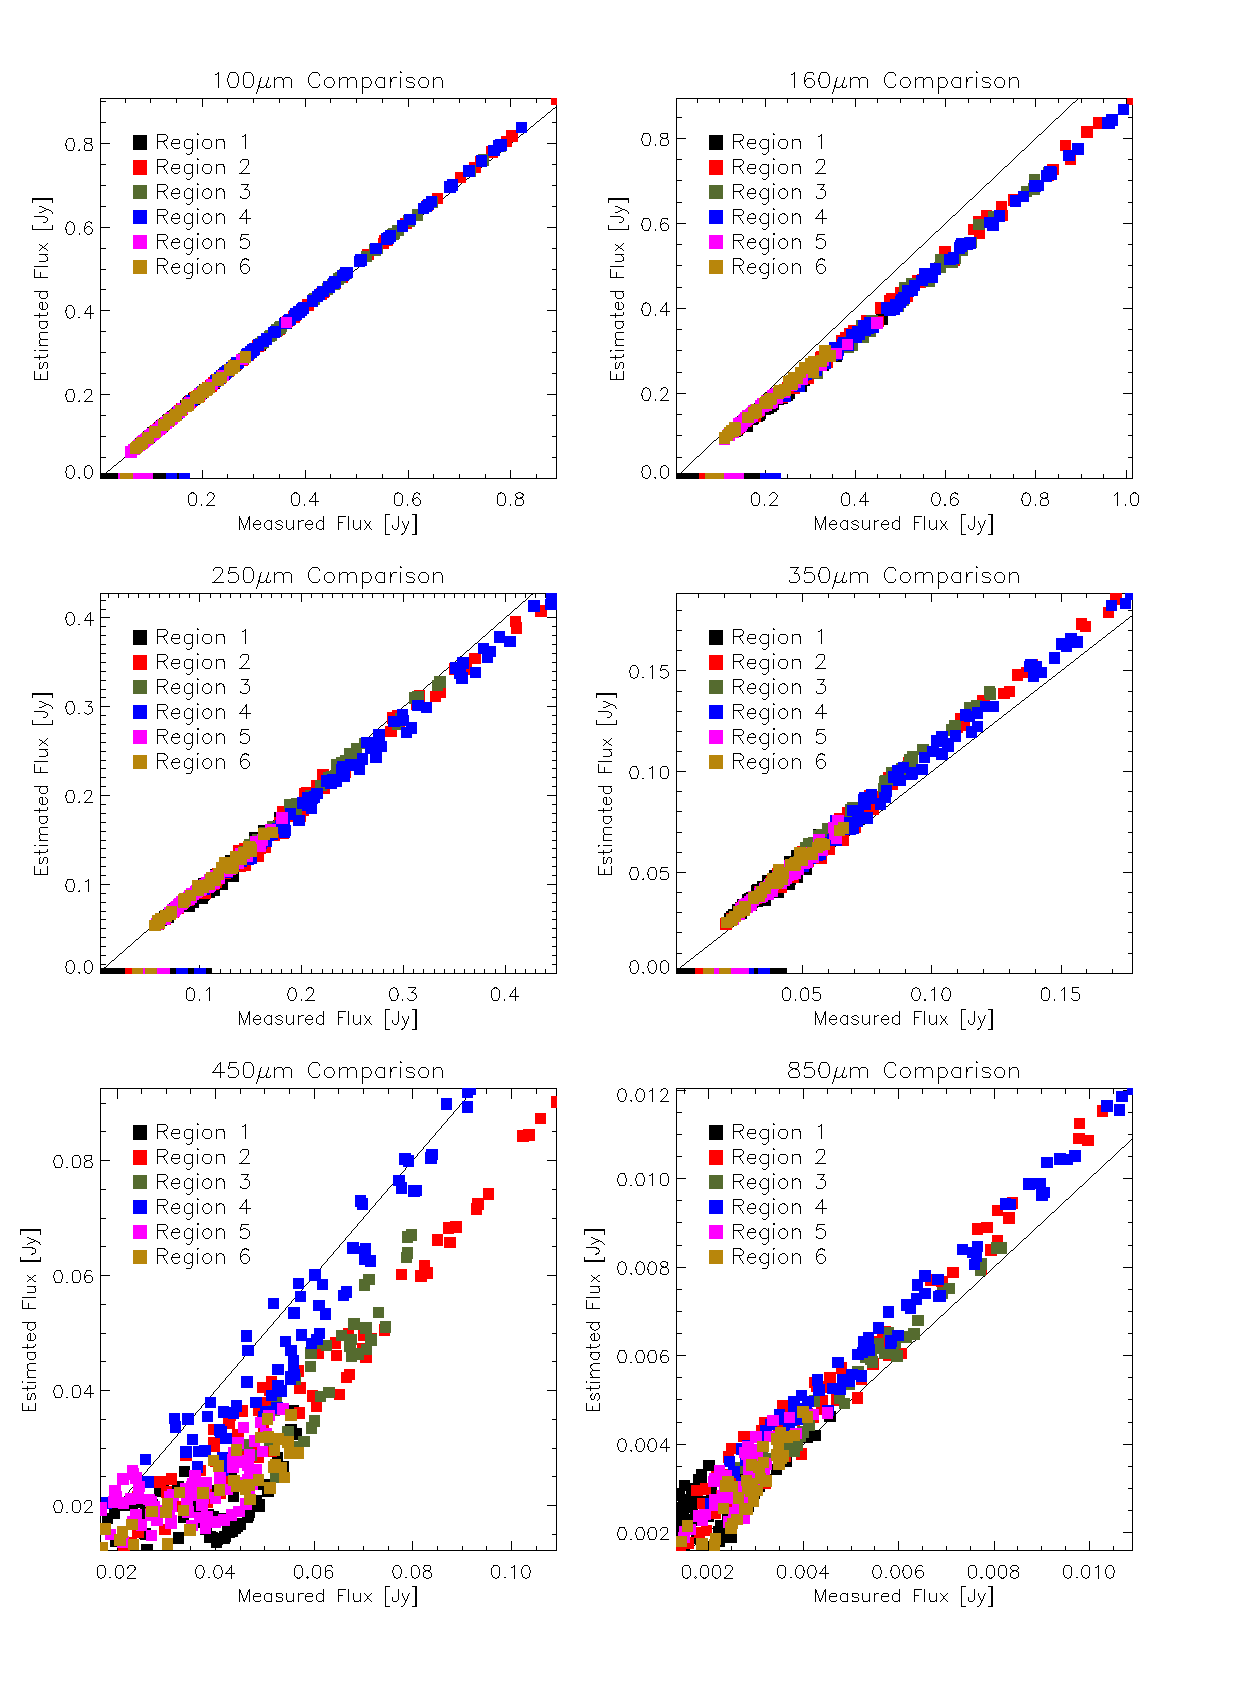
\includegraphics[width=1.\textwidth]{sed_imgs/flux_compare_1_4.eps}
%  \caption[Planck Model SED Fit Quality Using 450$\mu$m Data]{Quality of the SED fits to the Planck model using the 450$\mu$m emission.  The regions shown are the regions in figure \ref{fig:regions}.}
%  \label{fig:w1_4}
%\end{figure}


%\begin{figure}
%  \centering
%  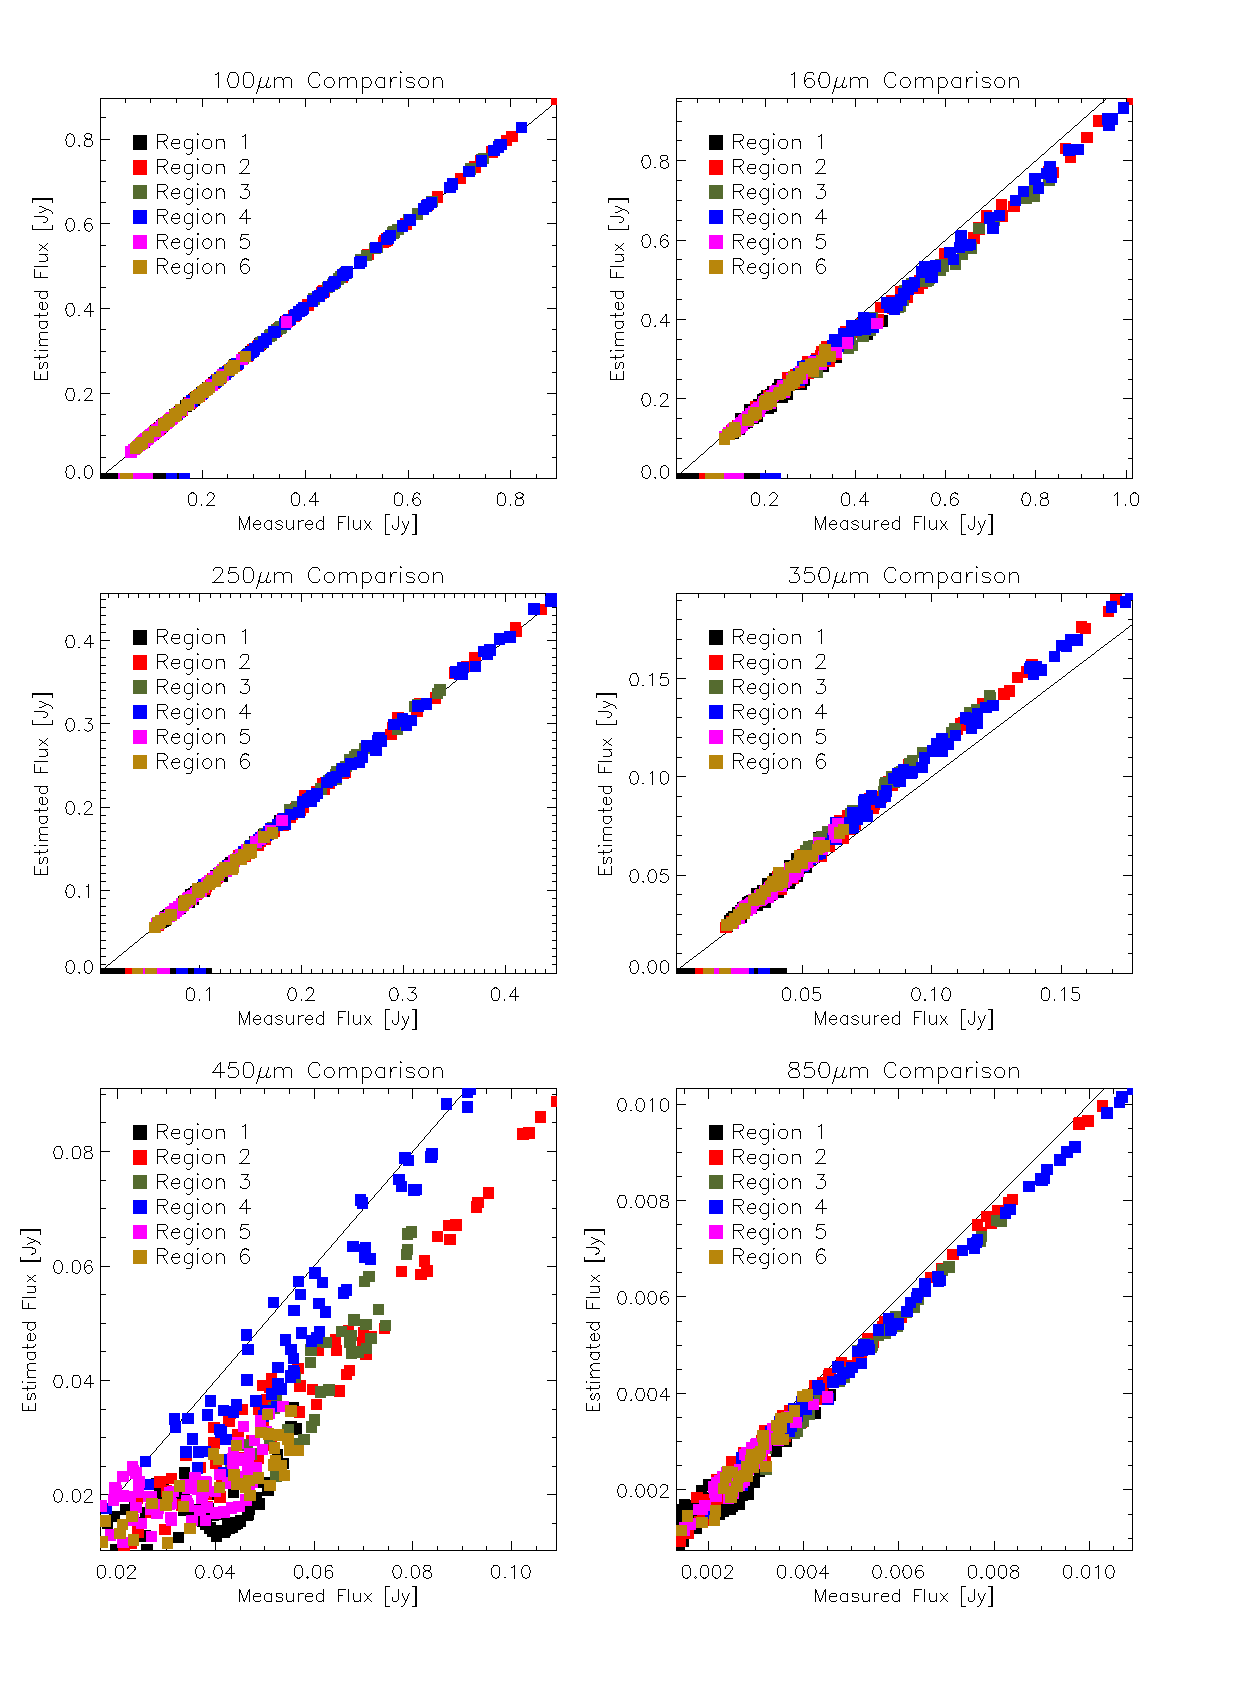
\includegraphics[width=1.\textwidth]{sed_imgs/flux_compare_free_4.eps}
%  \caption[Emissivity as a Free Parameter SED Fit Quality Using 450$\mu$m Data]{Quality of the SED fits with the dust emissivity index as a free parameter using the 450$\mu$m emission.  The regions shown are the regions in figure \ref{fig:regions}.}
%  \label{fig:wf_4}
%\end{figure}
